% Statuses:
% 0 - not started
% 1 - started, ideas collected
% 2 - less than half the length
% 3 - half the length
% 4 - full length, may need rephrasing
% 5 - done
% ==============================================================================
\chapter{Introduction}
% STATUS: 3
% motivation - longer
% how I solved it, avoid first person
% overview which chapter solves what

% establish your territory
%   state the general topic and give some background
%   provide a review of the literature related to the topic
%   define the terms and scope of the topic
\emph{Security-Enhanced Linux} (SELinux) is a~mandatory access control mechanism
used in Linux distributions. It extends the traditional file permissions using a
security policy that cannot be overridden by users. The \emph{audit2allow}
utility is one of several tools used by system administrators to troubleshoot
SELinux denials. Security policy developers use audit2allow to create a~basis
for security policy modules for their products. The audit2allow utility analyzes
SELinux denials and generates policy rules that can be loaded into the security
policy to allow the operations that were previously denied.

% establish a~niche
%   outline the current situation
%   evaluate the current situation (advantages/ disadvantages) and identify the gap
In certain situations, the audit2allow utility fails to provide effective and
secure solution. The utility was designed to solve problems caused by missing
rules in security policy, but users often use audit2allow to solve problems that
should not be solved by adding new rules to the policy. As a~result, users end
up with policy rules that give processes too much permissions, making whole
system more vulnerable.

In other situations, the audit2allow utility provides nonfunctional solutions
because it is not aware of recently added features of SELinux. There are new
policy statements that provide more granular control over given permissions. The
audit2allow utility is unable to detect that the denial was caused by these
statement and fails to provide working solution. Security policy developers
cannot use the audit2allow utility to generate these statements.

% introduce the current research
%   identify the importance of the proposed research
Users that are not familiar with SELinux cannot recognize limitations of the
audit2allow utility. They either fail to solve the problem or end up with
workaround that is potentionally unsecure.
%   state the research problem/ questions
%   state the research aims and/or research objectives
This thesis aims to analyze different causes of SELinux denials and evaluate the
quality of solutions provided by the audit2allow utility. Situations that are
best resolved using other tools should be detected by audit2allow and user
should be warned. Support for new SELinux features should be added to
audit2allow. As a~part of thesis, two new features were implemented.
%   state the hypotheses

%   outline the order of information in the thesis
Second chapter of the thesis presents Security-Enhanced Linux, introduces
SELinux policy language, describes auditing of security events, and provides
detailed description of the audit2allow utility. The third chapter analyzes
situations where the audit2allow utility generates nonfunctional or unsecure
solutions. The fourth chapter goes through implementation details of selected
improvements to audit2allow. The fifth chapter describes unit and integration
tests of implemented improvements to audit2allow.
%   outline the methodology

% ==============================================================================
\chapter{Security-Enhanced Linux and audit2allow}
% STATUS: 4
% describe SELinux, describe audit2allow, use examples, what are the
% problems of SELinux. Purpose of audit2allow, how is it used, how does it work,
% internal structure of audit2allow.

This chapter describes basic concepts of Security-Enhanced Linux, introduces the
SELinux security policy language, provides overview of the Linux Audit System,
and describes in detail the audit2allow utility.

% ------------------------------------------------------------------------------
% TOPIC: SELinux introduction and motivation
% ----------------------------------------
% STATUS: 4
% 2.1 INTRODUCTION                                                      Y
%     2.1.1 Is SELinux useful                                           Y
% 1. Introduction
%     1.1. Benefits of running SELinux
%     1.2. Examples
\section{Security-Enhanced Linux}
Security-Enhanced Linux (SELinux) is a~mandatory access control mechanism that
consists of kernel modifications and user-space tools and is a~part of several
Linux distributions.

\subsection{Purpose of SELinux}
Without SELinux, operating system relies on traditinal access control methods
such as file permissions. Users can grant insecure file permissions to others or
gain access to files that they do not need \cite{selinuxguide}:
\begin{itemize}
    \item Users can reveal sensitive information by setting world readable
        permissions on their files. For example, they can set read permission
        for everyone on SSH keys in the \texttt{\textasciitilde/.ssh/}
        directory.
    \item Processes can change security properties. For example, mail client can
        make user's mail readable by other users.
    \item Processes inherit user's rights. For example, every application, even
        though it may be compromised, is able to read all user's files.
\end{itemize}

SELinux enforces a~security policy that cannot be overriden by users.
Application are allowed to perform only actions they need for normal operation,
everything else is denied by default. Applications do not need to be aware of
SELinux. When an action is denied, it is reported via ``access denied'' error
code to the application \cite{centoshowto}.

%\subsection{How Does SELinux Enforce a~Security Policy}
%
%\begin{figure}
%    \centering
%    \label{fig:policyenforcing}
%    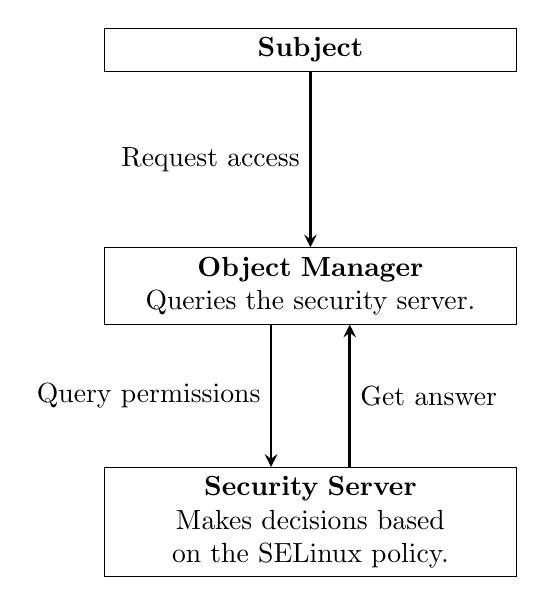
\begin{tikzpicture}
    \usetikzlibrary{calc}
    \tikzstyle{line} = [->,>=stealth, line width=1pt]
    \tikzstyle{rec} = [rectangle, draw=black, align=center, text width=5cm]

    \node(subject) [rec] {\textbf{Subject}};
    \node(objman) [rec, below of=subject, node distance=3cm] {\textbf{Object
    Manager}\\ Queries the security server.};
    \node(secser) [rec, below of=objman, node distance=3cm]
    {\textbf{Security Server}\\ Makes decisions based on the SELinux
    policy.};

    \draw[line] (subject) -- node[midway,left] {Request access} (objman);
    \draw[line] ([xshift=-0.5cm]objman.south) -- node[midway,left] {Query
    permissions} ([xshift=-0.5cm]secser.north);
    \draw[line] ([xshift=0.5cm]secser.north) -- node[midway,right] {Get
    answer} ([xshift=0.5cm]objman.south);
\end{tikzpicture}

%    \caption{High-level process of policy enforcing}
%\end{figure}
%
%The high-level process of policy enforcing (see figure~\ref{fig:policyenforcing}):
%\begin{enumerate}
%    \item A \emph{subject} wants to perform an action upon an \emph{object}.
%    \item An \emph{Object Manager} queries the \emph{Security Server} for a
%    decision.
%    \item \emph{Security Server} consults the \emph{Security Policy}
%    and makes decision to allow or deny the action.
%\end{enumerate}
%
%For example, when process \texttt{httpd} wants to open the
%\texttt{/etc/httpd/conf/httpd.conf} file, security server in kernel allows the
%operation. It is desirable to allow \texttt{httpd} access its configuration
%files, so the SELinux policy contains rules that allow this operation. But if
%process \texttt{httpd} would want to write to the \texttt{/etc/passwd} file, the
%operation would be denied. Process \texttt{httpd} should not change the
%\texttt{/etc/passwd} file, so the rules which would allow this operation are not
%present in policy.

% ----------------------------------------
% TOPIC: SELinux components
% ----------------------------------------
% STATUS: 4
% 2.2 CORE SELINUX COMPONENTS                                           Y
%     1.3. SELinux Architecture
\subsection{SELinux Components}
SELinux is composed of kernel and userspace part \cite[pp.~19--22]{tsn}. Main
components of SELinux, are shown in figure \ref{fig:selinuxcomponents}.

\begin{figure}
    \centering
    \label{fig:selinuxcomponents}
    % COUNT: 510
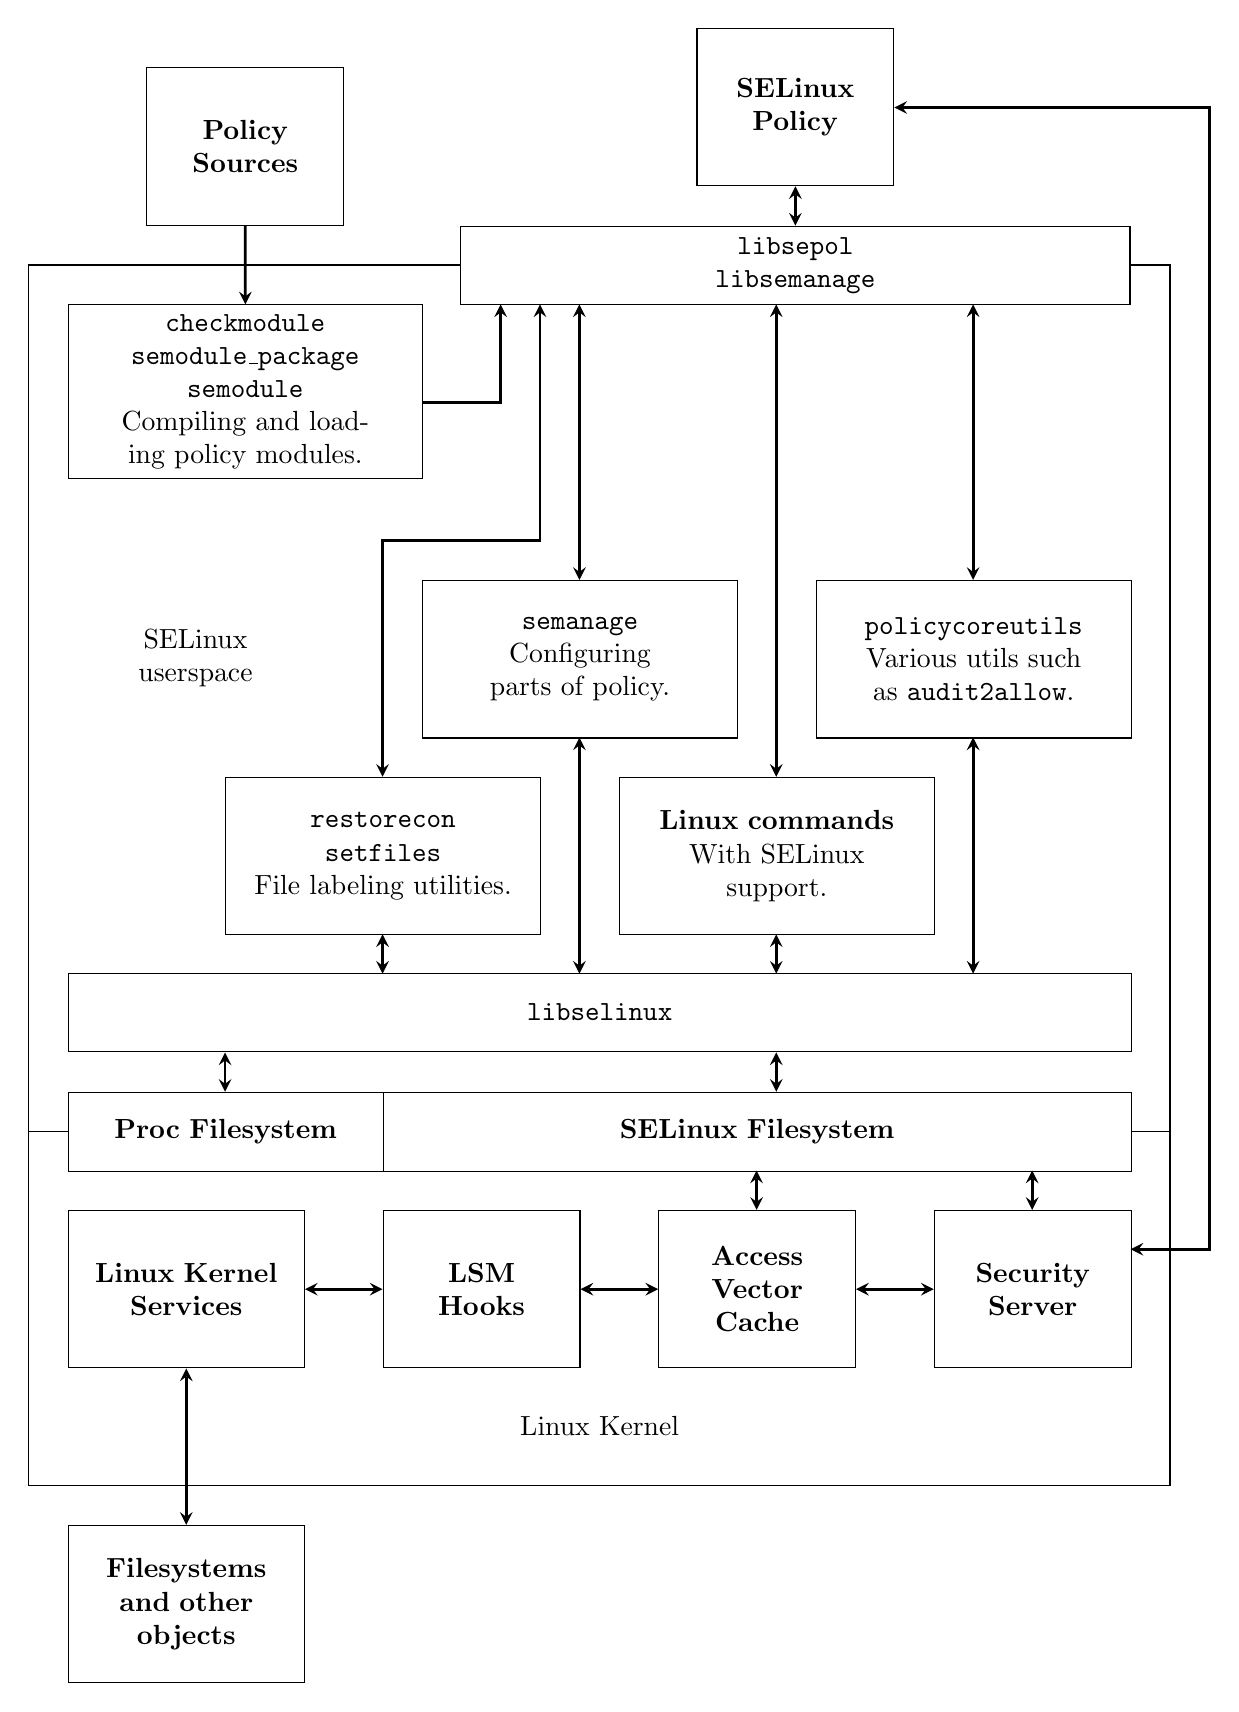
\begin{tikzpicture}
    \usetikzlibrary{calc}
    \tikzstyle{arrow} = [->,>=stealth, line width=1pt]
    \tikzstyle{darrow} = [<->,>=stealth, line width=1pt]
    \tikzstyle{rec} = [rectangle, draw=black, align=center, text width=3.5cm,
        minimum height=2cm, minimum width=4cm, fill=white]

    \draw (0,0) rectangle (14.5,-11);
    \draw (0,-11) rectangle (14.5,-15.5);

    \node(userspace) [rectangle, text width=2cm, align=center]
        at (1,-4.5) [anchor=north west]
        {SELinux userspace};
    \node(kernel) [rectangle, text width=4cm, minimum width=13.5cm,
        align=center]
        at (0.5,-14.5) [anchor=north west]
        {Linux Kernel};

    \node(policysource) [rec, text width=2cm, minimum width=2.5cm]
        at (1.5,0.5) [anchor=south west]
        {\textbf{Policy Sources}};
    \node(compiling) [rec, text width=4cm, minimum width=4.5cm]
        at (0.5,-0.5) [anchor=north west]
        {\textbf{\texttt{checkmodule}\\ \texttt{semodule\_package}\\
        \texttt{semodule}}\\ Compiling and loading policy modules.};
    \node(libsepol) [rec, text width=8cm, minimum width=8.5cm, minimum
        height=1cm]
        at (14,0.5) [anchor=north east]
        {\textbf{\texttt{libsepol}\\ \texttt{libsemanage}}};
    \node(policy) [rec, text width=2cm, minimum width=2.5cm]
        at (11,1) [anchor=south east]
        {\textbf{SELinux Policy}};
    \node(semanage) [rec]
        at (5,-4) [anchor=north west]
        {\textbf{\texttt{semanage}}\\ Configuring parts of policy.};
    \node(policycoreutils) [rec, right of=semanage, node distance=5cm]
        {\textbf{\texttt{policycoreutils}}\\ Various utils such as
        \texttt{audit2allow}.};
    \node(restorecon) [rec]
        at (2.5,-6.5) [anchor=north west]
        {\textbf{\texttt{restorecon}\\ \texttt{setfiles}}\\ File labeling
        utilities.};
    \node(linuxcmd) [rec, right of=restorecon, node distance=5cm]
        {\textbf{Linux commands}\\ With SELinux support.};
    \node(libselinux) [rec, text width=13cm, minimum width=13.5cm, minimum
        height=1cm]
        at (0.5,-10) [anchor=south west]
        {\textbf{\texttt{libselinux}}};
    \node(selinuxfs) [rec, text width=9cm, minimum width=9.5cm, minimum
        height=1cm]
        at (4.5,-10.5) [anchor=north west]
        {\textbf{SELinux Filesystem}};
    \node(procfs) [rec, text width=3.5cm, minimum width=4cm, minimum
        height=1cm]
        at (0.5,-10.5) [anchor=north west]
        {\textbf{Proc Filesystem}};
    \node(kernelservices) [rec, text width=2.5cm, minimum width=3cm]
        at (0.5,-12) [anchor=north west]
        {\textbf{Linux Kernel Services}};
    \node(fs) [rec, text width=2.5cm, minimum width=3cm,
        below of=kernelservices, node distance=4cm]
        {\textbf{Filesystems and other objects}};
    \node(lsmhooks) [rec, text width=2cm, minimum width=2.5cm,
        right of=kernelservices, node distance=3.75cm]
        {\textbf{LSM Hooks}};
    \node(avc) [rec, text width=2cm, minimum width=2.5cm, right of=lsmhooks,
        node distance=3.5cm]
        {\textbf{Access Vector Cache}};
    \node(secser) [rec, text width=2cm, minimum width=2.5cm, right of=avc,
        node distance=3.5cm]
        {\textbf{Security Server}};

    \draw[arrow] (policysource) -- (compiling);
    \draw[darrow] (libsepol) -- (policy);
    \draw[darrow] (fs) -- (kernelservices);
    \draw[darrow] (kernelservices) -- (lsmhooks);
    \draw[darrow] (lsmhooks) -- (avc);
    \draw[darrow] (avc) -- (secser);

    \draw[arrow] (5,-1.75) -- (6,-1.75) -- (6,-0.5);
    \draw[darrow] (6.5,-0.5) -- (6.5,-3.5) -- (4.5,-3.5) -- (4.5,-6.5);
    \draw[darrow] (9.5,-0.5) -- (9.5,-6.5);
    \draw[darrow] (7,-0.5) -- (7,-4);
    \draw[darrow] (12,-0.5) -- (12,-4);
    \draw[darrow] (4.5,-8.5) -- (4.5,-9);
    \draw[darrow] (7,-6) -- (7,-9);
    \draw[darrow] (9.5,-8.5) -- (9.5,-9);
    \draw[darrow] (12,-6) -- (12,-9);

    \draw[darrow] (2.5,-10) -- (2.5,-10.5);
    \draw[darrow] (9.5,-10) -- (9.5,-10.5);
    \draw[darrow] (9.25,-11.5) -- (9.25,-12);
    \draw[darrow] (12.75,-11.5) -- (12.75,-12);
    \draw[darrow] (14,-12.5) -- (15,-12.5) -- (15,2) -- (11,2);
\end{tikzpicture}

    % TODO: add "adapted from"?
    \caption{Main SELinux components.}
\end{figure}

\begin{description}
    \item [libsepol and libsemanage] Libraries for working with SELinux binary
        policy and policy infrastructure. The libsepol library is used for
        example for loading policy modules into the active security policy. The
        libsemanage library is used for example for assigning security contexts
        to TCP or UDP ports.
    \item [libselinux] API for implementing SELinux-aware applications. For
        example, SELinux-aware window manager can use the libselinux library to
        compute security contexts of its objects.
    \item [checkmodule, semodule\_package, semodule] Utilities that compile
        SELinux policy and load it into the kernel.
    \item [semanage] Utility for configuring various parts of policy, for
        example setting contexts for TCP and UDP ports. It uses mainly the
        libsemanage library.
    \item [restorecon and setfiles] Utilities for restoring default context of
        files (see section \ref{filecontexts}).
    \item [policycoreutils] Various utilities for working with and
        troubleshooting of SELinux, for example the audit2allow utility
        described in section \ref{audit2allow}.
    \item [Modified Linux Commands] Standard Linux commands such as ls or ps,
        modified to support SELinux.
    \item [SELinux and proc filesystem] Userspace tools communicate with kernel
        security server via the \texttt{/proc} and \texttt{/sys/fs/selinux}
        filesystem.
    \item [Security Server] Makes security decisions. It is embedded in the
        kernel and it obtains the security policy via userspace tools. Security
        server does not enforce the decision, it only states whether the
        operation is allowed or not.
    \item [Access Vector Cache] Caches security decision made by security
        server.
    \item [Linux Security Module Hooks] Call SELinux Security Server.
\end{description}

% ------------------------------------------------------------------------------
\section{Basic Concepts}
% STATUS: 4

This section defines basic terms related to SELinux, such as mandatory access
control, type enforcement, multi-level and multi-category security, security
context, and others.

% ----------------------------------------
% TOPIC: Subjects and objects
% ----------------------------------------
% STATUS: 4
\subsection{Subjects and Objects}
There are two basic entities in SELinux \cite[p.~29]{tsn}:
\begin{description}
    \item [Subject] is an entity that causes information to flow among objects
        or changes the system state. Within SELinux, a~subject is an active
        process that can access objects. A~process can also be an object, for
        example when a~process is sending signal to another process, the process
        receiving the signal is treated as an object.
    \item [Object] is a~system resource such as file, socket, pipe, TCP or UDP
        port, network interface, semaphore or shared memory segment.
\end{description}

% ----------------------------------------
% TOPIC: MAC, DAC
% ----------------------------------------
% STATUS: 4
% 2.3 MANDATORY ACCESS CONTROL (MAC)                                    Y
\subsection{Mandatory Access Control}

SELinux provides mandatory access control mechanism that extends the
discretionary access control mechanisms present in Linux kernel.

\subsubsection{Discretionary Access Control}
\emph{Discretionary access control} (DAC) is defined by \emph{Trusted Computer
System Evaluation Criteria} (TCSEC) standard \cite{orangebook}. System with DAC
must enable users to protect their data by controlling access to their data,
e.g. by setting permissions for other users or user groups. In DAC, users make
security decisions by specifying who can access their data. The disadvantage is
that users can propagate sensitive information.

Linux implements discretionary access control. Every object has an owner that
controls access to that object. Permissions are set in three scopes: user,
group, and others. For each scope, permissions to read, write, and execute can
be set.

\subsubsection{Mandatory Access Control}
\emph{Mandatory access control} (MAC), defined by TCSEC standard, provides more
restrictions than DAC. In this type of access control, operating system can
prevent subjects from performing operations on objects. This is achieved by
attaching subjects and objects set of security attributes. When a~subject
(usually a~process) wants to perform an operation on an object (file, directory,
socket, etc.), operating system first examines these attributes. Security
policy is then used to determine whether this operation should be allowed or
not. When using MAC, users do not have the ability to override the security
policy and, for example, propagate sensitive information.

There are several implementations of MAC. Linux kernel currently contains
several security modules implemented using \emph{Linux Security Modules} (LSM)
framework \cite{lsmusage}. Security-Enhanced Linux, developed by National
Security Agency and Red Hat \cite{selinuxcontr}, is used in Red Hat Enterprise
Linux (RHEL), CentOS, Fedora, and Android
\cite{selinuxguide,selinuxguidefedora,selinuxandroid}. AppArmor developed by
SUSE, is used in SUSE Linux Enterprise, openSUSE and Ubuntu
\cite{apparmor,apparmorubuntu}. There are two other Linux security modules,
Smack and TOMOYO Linux.

\subsection{SELinux and MAC Checks}
SELinux security checks are carried out after standard Linux DAC checks. When
running an SELinux-enabled system, when a~userspace process makes a~system call,
standard file permissions are checked first. Then, if the access is allowed, the
Linux Security Module hooks calls security checks in SELinux.

% ----------------------------------------
% TOPIC: SELinux users
% ----------------------------------------
% STATUS: 4
% 2.4 SELINUX USERS                                                     ?
\subsection{SELinux Users}
\label{selinuxuser}
SELinux uses its own user names that are different from standard Linux user
names \cite[p.~24]{tsn}. Every Linux user is associated to an SELinux user. For
example, Linux user \texttt{root} is mapped to SELinux user
\texttt{unconfined\_u} on Fedora 27. There is a~special SELinux user that is
not mapped to any user: \texttt{system\_u}.

Available SELinux users can be listed using the \texttt{seinfo -{}-user}
command:
\begin{lstlisting}
$ seinfo --user

Users: 8
   guest_u
   root
   staff_u
   sysadm_u
   system_u
   unconfined_u
   user_u
   xguest_u
\end{lstlisting}

% ----------------------------------------
% TOPIC: RBAC
% ----------------------------------------
% STATUS: 4
% 2.5 ROLE-BASED ACCESS CONTROL (RBAC)                                  ?
\subsection{Role-Based Access Control}
\label{rbac}
SELinux uses role-based access control (RBAC) as one of its security mechanisms.
RBAC as general concept is based on users, roles, and permissions, and
relationships between them. RBAC defines the role-permission, user-role, and
role-role relationships.

In SELinux, every user is associated to one or more roles \cite[p.~24]{tsn}.
Each role can access only types that are associated to that role. For example,
user \texttt{system\_u} is associated to roles \texttt{unconfined\_r} and
\texttt{system\_r} on Fedora 27.

Available SELinux roles can be listed using the \texttt{seinfo -{}-role}
command:
\begin{lstlisting}
$ seinfo --role

Roles: 14
   auditadm_r
   dbadm_r
   guest_r
   logadm_r
   nx_server_r
   object_r
   secadm_r
   staff_r
   sysadm_r
   system_r
   unconfined_r
   user_r
   webadm_r
   xguest_r
\end{lstlisting}

% ----------------------------------------
% TOPIC: TE
% ----------------------------------------
% STATUS: 4
% 2.6 TYPE ENFORCEMENT (TE)                                             Y
%     2.6.1 Constraints                                                 ?
%     2.6.2 Bounds                                                      N
\subsection{Type Enforcement}
\label{te}
SELinux uses type enforcement for enforcing mandatory access control
\cite[pp.~25--26]{tsn}. All subjects and objects have a~type associated.
Processes running with the same type are called a~\emph{domain}. SELinux
policy then contains rules that allow domains access types.

Available SELinux types can be listed using the \texttt{seinfo -{}-type}
command:
\begin{lstlisting}
$ seinfo --type

Types: 4845
   abrt_t
   alsa_t
   antivirus_t
   bin_t
   cluster_t
   crond_t
   ...
\end{lstlisting}

% ----------------------------------------
% TOPIC: MLS and MCS
% ----------------------------------------
% STATUS: 4
%     4.13. Multi-Level Security (MLS)
%         4.13.1. MLS and System Privileges
%         4.13.2. Enabling MLS in SELinux
%         4.13.3. Creating a~User With a~Specific MLS Range
%         4.13.4. Setting Up Polyinstantiated Directories
\subsection{Multi-Level and Multi-Category Security}
\label{mls}
In addition to type enforcement and role-based access control, SELinux also
supports multi-level security (MLS) and multi-category security (MCS)
\cite[pp.~48--53]{tsn}. For the purposes of MLS and MCS, security context is
extended by level or range entry.

Security levels conform to the Bell-LaPadula model. For processes, security
levels describe subjects clearance, for objects, they describe objects
classification. Process running at certain security level can:
\begin{itemize}
    \item read and write at their current level,
    \item read only at lower levels,
    \item write only at higher levels.
\end{itemize}
This means that processes cannot read data with higher security level and
cannot leak sensitive information to the lower levels. Multi-level security is
not used by default in most SELinux-enabled Linux distributions such as Fedora
or RHEL, but it is supported.

% ----------------------------------------
% TOPIC: SELinux context
% ----------------------------------------
% STATUS: 4
% 2.7 SECURITY CONTEXT                                                  Y
% 2. SELinux Contexts
\subsection{SELinux Security Context}
\label{context}
Security decisions are based on a~\emph{security context} that must be assigned
to every subject and object \cite[pp.~27--28]{tsn}. The security context is
sometimes reffered to as \emph{security label} or just \emph{label}.  The
security context is a~string in the following form:
\begin{lstlisting}
user:role:type[:range]
\end{lstlisting}
Where:
\begin{description}
    \item [\texttt{user}] The SELinux user (see section \ref{selinuxuser}).
    \item [\texttt{role}] The SELinux role used by role-based access control
        (see section \ref{rbac}).
    \item [\texttt{type}] The SELinux type used by type enforcement (see section
        \ref{te}).
    \item [\texttt{range}] Used by MLS or MCS (see section \ref{mls}). It is optional.
\end{description}

Example of subject security contexts:
\begin{lstlisting}
$ ps -eZ
LABEL                             PID TTY          TIME CMD
system_u:system_r:init_t:s0         1 ?        00:00:04 systemd
system_u:system_r:kernel_t:s0       2 ?        00:00:00 kthreadd
system_u:system_r:auditd_t:s0    1139 ?        00:00:00 auditd
system_u:system_r:alsa_t:s0      1164 ?        00:00:00 alsactl
...
\end{lstlisting}

Example of object security contexts:
\begin{lstlisting}
$ ls -Z /etc
               system_u:object_r:etc_t:s0 alsa
         system_u:object_r:cupsd_etc_t:s0 cups
          system_u:object_r:dhcp_etc_t:s0 dhcp
       system_u:object_r:passwd_file_t:s0 passwd
          system_u:object_r:net_conf_t:s0 resolv.conf
...
\end{lstlisting}

% ----------------------------------------
% TOPIC: subjects and objects, object classes, permissions, allow rule
% ----------------------------------------
% STATUS: 4
% 2.8 SUBJECTS                                                          Y
% 2.9 OBJECTS                                                           Y
%     2.9.1 Object Classes and Permissions                              Y
%     2.9.2 Allowing a~Process Access to Resources                      Y
% 4.10 OBJECT CLASS AND PERMISSION STATEMENTS                           Y
%     4.10.1 class                                                      Y
%     4.10.2 Associating Permissions to a~Class                         Y
%     4.10.3 common                                                     Y
%     4.10.4 class                                                      Y
\subsection{Object Classes}
Each object belongs to an object class. Object classes specify operations that
can be performed on the object \cite[pp.~29--30]{tsn}. For example, on Fedora
27, there are the following classes:
\begin{lstlisting}
$ seinfo --class

Classes: 97
   blk_file
   chr_file
   dbus
   dir
   fd
   file
   filesystem
   ipc
   ...
\end{lstlisting}

Each class is associated to a~set of permissions. For example, on Fedora 27,
class \texttt{node} provides the following permissions:
\begin{lstlisting}
$ seinfo --class node -x

Classes: 1
   class node
{
	dccp_send
	enforce_dest
	tcp_recv
	rawip_send
	tcp_send
	udp_recv
	dccp_recv
	sendto
	udp_send
	recvfrom
	rawip_recv
}
\end{lstlisting}
SELinux object classes maps to the kernel object classes (files, sockets, etc.)
and userspace objects (for X-Windows or D-Bus).

% ----------------------------------------
% TOPIC: labeling
% ----------------------------------------
% STATUS: 4
%     2.9.3 Labeling Objects                                            Y
%         2.9.3.1 Labeling Extended Attribute Filesystems               Y
%             2.9.3.1.1 Copying and Moving Files                        Y
%         2.9.3.2 Labeling Subjects                                     Y
%     2.9.4 Object Reuse                                                N
% 2.10 COMPUTING SECURITY CONTEXTS                                      Y
%     2.10.1 Security Context Computation for Kernel Objects            Y
%         2.10.1.1 Process                                              Y
%         2.10.1.2 Files                                                Y
%         2.10.1.3 File Descriptors                                     N
%         2.10.1.4 Filesystems                                          N
%         2.10.1.5 Network File System (nfsv4)                          N
%         2.10.1.6 INET Sockets                                         N
%         2.10.1.7 IPC                                                  N
%         2.10.1.8 Message Queues                                       N
%         2.10.1.9 Semaphores                                           N
%         2.10.1.10 Shared Memory                                       N
%         2.10.1.11 Keys                                                N
%     2.10.2 Using libselinux Functions                                 N
%         2.10.2.1 avc_compute_create and security_compute_create       N
%         2.10.2.2 avc_compute_member and security_compute_member       N
%         2.10.2.3 security_compute_relabel                             N
%     2.2. SELinux Contexts for Processes
%     2.3. SELinux Contexts for Users
\subsection{Labeling Subjects and Objects}
Security contexts for subjects and objects are computed by the kernel security
server using several policy statements \cite[pp.~31--33]{tsn}.

\subsubsection{Labeling Processes}
The first init process usually transitions to its own unique domain, for example
\texttt{init\_t}. On fork, the child process inherits the security context of
its parent. On exec, the child process may transition to different security
context. This is achieved by type transition policy statements. SELinux-aware
processes may change context by calling \texttt{setcon()} or
\texttt{setexeccon()} functions from the libselinux library.

\subsubsection{Labeling Files}
Security context for files is computed as follows:
\begin{description}
    \item [\texttt{user}] User is inherited from the creating process.
    \item [\texttt{role}] Role defaults to \texttt{object\_r} unless modified by
        \texttt{role\_transition} statement.
    \item [\texttt{type}] Type defaults to the type of the parent directory
        unless modified by \texttt{type\_transition} statement.
\end{description}
File contexts are covered in depth in section \ref{filecontexts}.

% ----------------------------------------
% TOPIC: type transitions
% ----------------------------------------
% STATUS: 4
% 2.12 DOMAIN AND OBJECT TRANSITIONS                                    Y
%     2.12.1 Domain Transition                                          Y
%         2.12.1.1 Type Enforcement Rules                               Y
%     2.12.2 Object Transition                                          Y
%     2.1. Domain Transitions
%     4.14. File Name Transition
\subsection{Type Transitions}
\label{typetransitions}
To run different processes in different domains, we need a~way how to
\emph{transition} a~process from one domain to another. To attach specific label
to an object, we need to transition an object from one type to another. Both
transitions can be achieved using the \texttt{type\_transition} statement.

\subsubsection{Domain Transition}
Starting new process with different security context is called domain transition
\cite[pp.~43--47]{tsn}. For example, \texttt{systemd} process running as
\texttt{init\_t} needs to start the Apache HTTP Server as \texttt{httpd\_t}.
Apache executables are labeled \texttt{httpd\_exec\_t}. The following policy
rule allows the transition:
\begin{lstlisting}[language=te]
type_transition init_t httpd_exec_t:process httpd_t;
\end{lstlisting}
The \texttt{systemd} process does not need to be aware of SELinux. The
\texttt{type\_transition} rule in the policy will cause the \texttt{exec} call
to automatically perform the transition. There are conditions that needs to be
met before a domain transition can happen:
\begin{enumerate}
    \item The source domain has permission to transition into the target domain.
        For example:
\begin{lstlisting}[language=te]
allow init_t httpd_t:process transition;
\end{lstlisting}
    \item The source domain has permission to read and execute the binary. For
        example:
\begin{lstlisting}[language=te]
allow init_t httpd_exec_t:file { execute read getattr };
\end{lstlisting}
    \item The context of the executable needs to be set as an entry point into
        the target domain. For example:
\begin{lstlisting}[language=te]
allow httpd_t httpd_exec_t:file entrypoint;
\end{lstlisting}
\end{enumerate}

\subsubsection{Object Transition}
When a~new object is created it inherits the security context of its parent.
When it is required that the object has different context, an object transition
must be used \cite[pp.~47--48]{tsn}. For example when an X server creates a~file
in the \texttt{/tmp} directory (which has context \texttt{tmp\_t}), it gets
context \texttt{user\_tmp\_t}. This is achieved by the following
\texttt{type\_transition} rule:
\begin{lstlisting}[language=te]
type_transition xserver_t tmp_t:file user_tmp_t;
\end{lstlisting}
The X server does not need to be aware of SELinux, the kernel computes the label
automatically.

% ----------------------------------------
% TOPIC: SELinux modes
% ----------------------------------------
% STATUS: 4
% 2.15 SELINUX PERMISSIVE AND ENFORCING MODES                           Y
%     1.4. SELinux States and Modes
\subsection{SELinux Modes of Operation}

SELinux has three modes of operation \cite{selinuxguide}. The default mode is
\emph{enforcing}. In this mode, everything which is not allowed by the policy is
denied. When a~process tries to perform an action which is not allowed by the
policy, it is logged. In \emph{permissive} mode, SELinux is not enforcing the
policy, it only logs actions. In \emph{disabled} mode, SELinux is turned off.

Running SELinux in permissive mode is useful for catching AVC denials that can
be analyzed using the audit2allow utility. To perform single task (for example
to save a~file), several SELinux checks are usually needed. When running in
enforcing mode, only the first denial would be logged and the troubleshooting
would be more difficult.

% ------------------------------------------------------------------------------
% TOPIC: Policy language
% ----------------------------------------
% STATUS: 4
% 4.1 INTRODUCTION                                                      Y
%     4.1.1 CIL Overview                                                Y
% 4.2 KERNEL POLICY LANGUAGE                                            Y
%     4.2.1 Policy Source Files                                         Y
%     4.2.2 Conditional, Optional and Require Statement Rules           Y
%     4.2.3 MLS Statements and Optional MLS Components                  N
%     4.2.4 General Statement Information                               Y
%     4.2.5 Section Contents                                            N
% 2.14 TYPES OF SELINUX POLICY                                          Y
%     2.14.1 Example Policy                                             N
%     2.14.2 Reference Policy                                           Y
%     2.14.3 Policy Functionality Based on Name or Type                 Y
%     2.14.4 Custom Policy                                              N
%     2.14.5 Monolithic Policy                                          Y
%     2.14.6 Loadable Module Policy                                     Y
%         2.14.6.1 Optional Policy                                      N
%     2.14.7 Conditional Policy                                         ?
%     2.14.8 Binary Policy                                              Y
%     2.14.9 Policy Versions                                            Y
\section{SELinux Policy}
\label{policy}
Security decisions made by the security server in kernel are made using
SELinux policy. This section describes the most important SELinux policy
statements. The primary output audit2allow utility are policy statements.

SELinux supports either monolithic (compiled from single source file) or modular
policy. Modular policy, which is used in Fedora and RHEL, consists of mandatory
base policy source file and loadable modules. In Fedora, almost every module
contains policy for one application or service, such as the \texttt{apache} or
\texttt{xserver} module. The audit2allow utility can be used to create a
loadable policy module.

SELinux policy statements starts with a~statement keyword usually followed by
several identifiers and semicolon at the end. Comments starts with a~``\#''.
Example of an allow rule:

\begin{lstlisting}[language=te]
# This is an allow rule
allow httpd_t httpd_exec_t: file { ioctl read getattr lock execute open };
\end{lstlisting}

% ----------------------------------------
% TOPIC: user, role and type statements
% ----------------------------------------
% STATUS: 4
% 4.3 POLICY CONFIGURATION STATEMENTS                                   ?
%     4.3.1 policycap                                                   ?
% 4.4 DEFAULT OBJECT RULES                                              Y
%     4.4.1 default_user                                                ?
%     4.4.2 default_role                                                ?
%     4.4.3 default_type                                                ?
%     4.4.4 default_range                                               ?
% 4.5 USER STATEMENTS                                                   ?
%     4.5.1 user                                                        ? 
% 4.6 ROLE STATEMENTS                                                   ?
%     4.6.1 role                                                        ?
%     4.6.2 attribute_role                                              ?
%     4.6.3 roleattribute                                               ?
%     4.6.4 allow                                                       ?
%     4.6.5 role_transition                                             ?
%     4.6.6 dominance                                                   ?
% 4.7 TYPE STATEMENTS                                                   Y
%     4.7.1 type                                                        Y
%     4.7.2 attribute                                                   Y
%     4.7.3 typeattribute                                               Y
%     4.7.4 typealias                                                   Y
%     4.7.5 permissive                                                  Y
%     4.7.6 type_transition                                             Y
%     4.7.7 type_change                                                 N
%     4.7.8 type_member                                                 N
% user role attribute_role roleattribute allow role_transition type
% attribute typeattribute
% user -- role -- type
% role - group: attribute_role, rule: roleattribute
% type - group: attribute, typeattribute

\subsection{User, Role and Type Statements}
\label{userroletype}
To support mechanisms such as type enforcement, role-based access control, and
multi-level and multi-category security, SELinux assigns subjects and objects
security contexts. Security context is combination of user, role, type, and
optionally range identifiers (see section \ref{context}). This section describes
policy statements that declare these identifiers.

SELinux users are declared using the \texttt{user} statement. Users are assigned
one or more roles. SELinux roles are declared using the \texttt{role} statement.
Roles are assigned types that they can access. SELinux types are declared using
the \texttt{type} statement.

\begin{figure}
    \centering
    \label{fig:userroletype}
    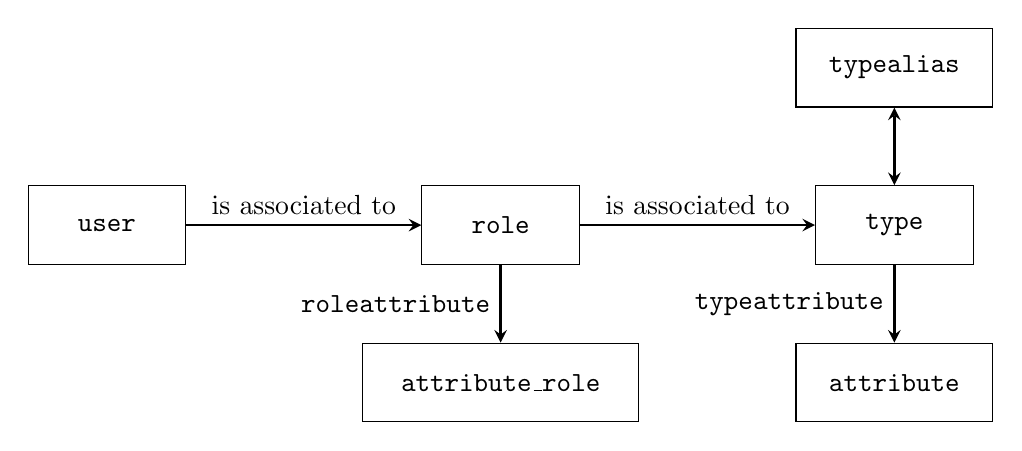
\begin{tikzpicture}
    \usetikzlibrary{calc}
    \tikzstyle{arrow} = [->,>=stealth, line width=1pt]
    \tikzstyle{darrow} = [<->,>=stealth, line width=1pt]
    \tikzstyle{rec} = [rectangle, draw=black, align=center, text width=3.5cm,
        minimum height=1cm, minimum width=4cm, fill=white]

    \node(user) [rec, text width=1.5cm, minimum width=2cm]
        at (0,-0.5) [anchor=north west]
        {\textbf{\texttt{user}}};

    \node(role) [rec, text width=1.5cm, minimum width=2cm]
        at (5,-0.5) [anchor=north west]
        {\textbf{\texttt{role}}};

    \node(type) [rec, text width=1.5cm, minimum width=2cm]
        at (10,-0.5) [anchor=north west]
        {\textbf{\texttt{type}}};

    \node(roleattr) [rec, text width=3cm, minimum width=3.5cm]
        at (4.25,-2.5) [anchor=north west]
        {\textbf{\texttt{attribute\_role}}};

    \node(typeattr) [rec, text width=2cm, minimum width=2.5cm]
        at (9.75,-2.5) [anchor=north west]
        {\textbf{\texttt{attribute}}};

    \node(typealias) [rec, text width=2cm, minimum width=2.5cm]
        at (9.75,1.5) [anchor=north west]
        {\textbf{\texttt{typealias}}};

    \draw[arrow] (user) -- node[pos=0.5,above] {is associated to} (role);
    \draw[arrow] (role) -- node[pos=0.5,above] {is associated to} (type);
    \draw[darrow] (typealias) -- (type);
    \draw[arrow] (role) -- node[pos=0.5,left] {\texttt{roleattribute}}
        (roleattr);
    \draw[arrow] (type) -- node[pos=0.5,left] {\texttt{typeattribute}}
        (typeattr);
\end{tikzpicture}

    \caption{Relationship of user, role, and type statements}
\end{figure}

Roles can be grouped together using the \texttt{attribute\_role} and
\texttt{roleattribute} statements. Types can be grouped together using the
\texttt{attribute} and \texttt{typeattribute} statements. Type aliases can be
defined using \texttt{typealias} statements. The relationship between various
statements is shown in figure \ref{fig:userroletype}.

\subsubsection{User Statements}
The \texttt{user} statement declares an identifier for an SELinux user. Syntax:
\begin{lstlisting}[language=te]
user seuser_id roles role_id;
\end{lstlisting}
Where:
\begin{description}
    \item [\texttt{seuser\_id}] SELinux user identifier.
    \item [\texttt{role\_id}] One or more role identifiers.
\end{description}
Example from Fedora 27:
\begin{lstlisting}[language=te]
user staff_u roles { system_r unconfined_r sysadm_r staff_r };
\end{lstlisting}

\subsubsection{Role Statements}
The \texttt{role} statement either declares an identifier for an SELinux role
and optionally associates a~role to one or more types. Syntax:
\begin{lstlisting}[language=te]
role role_id;
role role_id types type_id;
\end{lstlisting}
Where:
\begin{description}
    \item [\texttt{role\_id}] SELinux role identifier.
    \item [\texttt{type\_id}] One or more type identifiers.
\end{description}
Example from Fedora 27:
\begin{lstlisting}[language=te]
role auditadm_r types { auditadm_t auditadm_screen_t auditadm_su_t
    auditadm_sudo_t chkpwd_t updpwd_t exim_t auditctl_t auditd_t
    mailman_mail_t user_mail_t postfix_postdrop_t postfix_postqueue_t
    qmail_inject_t qmail_queue_t run_init_t user_tmp_t vlock_t };
\end{lstlisting}

\subsubsection{Type Statements}
The \texttt{type} statement declares an identifier for an SELinux type. Type
identifiers usually ends with '\texttt{\_t}' to distinguish them from attribute
identifiers. Syntax:
\begin{lstlisting}[language=te]
type type_id;
type type_id, attribute_id;
type type_id alias alias_id;
type type_id alias alias_id, attribute_id;
\end{lstlisting}
Where:
\begin{description}
    \item [\texttt{type\_id}] SELinux type identifier.
    \item [\texttt{alias\_id}] One or more optional aliases declared by the
        \texttt{typealias} statement. Multiple aliases must be enclosed in
        braces.
    \item [\texttt{attribute\_id}] One or more optional attributes declared by
        the \texttt{attribute} statement. Multiple attributes must be separated
        by comma.
\end{description}
Example from Fedora 27:
\begin{lstlisting}[language=te]
type httpd_sys_content_t alias { httpd_fastcgi_content_t
    httpd_httpd_sys_script_ro_t httpd_fastcgi_script_ro_t },
    httpdcontent, httpd_content_type, entry_type, exec_type, file_type,
    non_auth_file_type, non_security_file_type;
\end{lstlisting}

\subsubsection{Other Statements}
The \texttt{attribute\_role} statement declares an identifier for a~group of
role identifiers. Syntax:
\begin{lstlisting}[language=te]
attribute_role attribute_id;
\end{lstlisting}
The \texttt{roleattribute} statement associates roles to role attributes.
Syntax:
\begin{lstlisting}[language=te]
roleattribute role_id attribute_id;
\end{lstlisting}
The \texttt{attribute} statement declares an identifier for a~group of type
identifiers. Syntax:
\begin{lstlisting}[language=te]
attribute attribute_id;
\end{lstlisting}
The \texttt{typeattribute} statement associates types to attributes. Syntax:
\begin{lstlisting}[language=te]
typeattribute type_id attribute_id;
\end{lstlisting}
The \texttt{typealias} statement declares type aliases. Syntax:
\begin{lstlisting}[language=te]
typealias type_id alias alias_id;
\end{lstlisting}

% ----------------------------------------
% TOPIC: AV rules
% ----------------------------------------
% STATUS: 4
% 4.9 ACCESS VECTOR RULES                                               Y
%     4.9.1 allow                                                       Y
%     4.9.2 dontaudit                                                   Y
%     4.9.3 auditallow                                                  Y
%     4.9.4 neverallow                                                  Y
\subsection{Access Vector Rules}
\label{avrules}
The access vector rules support type enforcement within SELinux. They control
what access do processes get. The audit2allow utility generates access vector
rules as an output. The \texttt{allow} rule grants an access to an object.
Syntax:
\begin{lstlisting}[language=te]
allow source_type target_type:obj_class perm_set;
\end{lstlisting}
Where:
\begin{description}
    \item [\texttt{source\_type}] One or more type or attribute identifiers (see
        section \ref{userroletype}). This field identifies the subject that is
        performing the operation.
    \item [\texttt{target\_type}] One or more type or attribute identifiers.
        This field identifies the object that is being accessed. When the
        target type is same as the source type, \texttt{self} keyword can be
        used instead of target type.
    \item [\texttt{obj\_class}] One or more object classes (for example
        \texttt{file} or \texttt{tcp\_socket}).
    \item [\texttt{perm\_set}] One or more permissions (for example
        \texttt{read} or \texttt{connectto}).
\end{description}
Example:
\begin{lstlisting}[language=te]
allow httpd_t samba_share_t:file { getattr open read };
\end{lstlisting}
In this example, processes running as \texttt{httpd\_t} are allowed to
\texttt{getattr}, \texttt{open}, and \texttt{read} files labeled as
\texttt{samba\_share\_t}.

There are three other AV rules that follow the syntax pattern of the
\texttt{allow} rule:
\begin{description}
    \item [\texttt{dontaudit}] Stops auditing (logging) of denials. It is used
        when the denial is expected to happen and does not cause any issues. The
        \texttt{dontaudit} rules help to keep audit logs clean.
    \item [\texttt{auditallow}] Audits the event. The \texttt{auditallow} rule
        itself does not allow the operation, so the rule must appear together
        with standard \texttt{allow} rule.
    \item [\texttt{neverallow}] Compiler statement that stops compilation if
        this rule is found somewhere in policy. It is used for marking rules
        that may be unsecure.
\end{description}
Internally, access vectors defined by AV rules are stored in memory as bit
arrays that are 32~bits long. Because of this limitation, object classses cannot
have more than 32 different permissions. Extended permission AV rules were
introduced to overcome this issue.

% ----------------------------------------
% TOPIC: Extended permission AV rules
% ----------------------------------------
% STATUS: 4
\subsection{Extended Permission Access Vector Rules}
\label{extavrules}

Since policy version 30, there are extended permission access vector rules that
expand the permission sets. Standard access vector rules operates with 32~bit
permission sets, extended permission AV rules adds arbitrary number of 256~bit
increments. Extended permission AV rules are currently (as of policy version 31)
used only for ioctl whitelisting, but they provide generic tool that can be used
in future for more granular control over an operation~\cite{selinuxmailxperms}.

Support for extended permission AV rules by the audit2allow utility was
implemented as a~part of this thesis. Syntax of extended permission AV rules
\cite{xpermrules}:
\begin{lstlisting}[language=te]
rule_name source_type target_type : obj_class operation xperm_set;
\end{lstlisting}
Where:
\begin{description}
    \item [\texttt{rule\_name}] is one of the following: \texttt{allowxperm},
        \texttt{dontauditxperm}, \texttt{auditallowxperm}, or
        \texttt{neverallowxperm}. The meaning is same as with standard AV rules.
        The \texttt{allowxperm} rule allows the access, the
        \texttt{dontauditxperm} rule denies and logs the access, the
        \texttt{auditallowxperm} rule logs the access, and the
        \texttt{neverallowxperm} rules is a~compiler statement to prevent
        unsecure rules from appearing in policy.
    \item [\texttt{source\_type}, \texttt{target\_type}, \texttt{obj\_class}]
        are source type, target type, and object class, same as with standard AV
        rule.
    \item [\texttt{operation}] is a~single keyword defining the operation to be
        implemented by the rule. As of policy version 31, only the
        \texttt{ioctl} operation is supported. In contrast to permissions in
        standard access vector rules, each extended permission AV rule has only
        one operation (standard AV rules can have many permissions).
    \item [\texttt{xperm\_set}] are extended permissions represented by numeric
        values. The meaning of values depends on the operation. Values can be
        written in decimal or hexadecimal form, for example \texttt{42} or
        \texttt{0x2a}. Multiple values must be separated by space and enclosed
        in braces, for example \texttt{\{ 1 2 3 \}}. Value ranges are supported,
        for example \texttt{50-60} (both 50 and 60 are included in the range).
        To allow all values except for those explicitly listed, the complement
        operator can be used, for example \texttt{\textasciitilde \{ 1 2 3 \}}.
\end{description}

Example of an extended permission AV rule:
\begin{lstlisting}[language=te]
allowxperm my_app_t my_socket_t : tcp_socket ioctl { 20 30 0x40 50-60 };
\end{lstlisting}
This rule allows a~process running as \texttt{my\_app\_t} to call \texttt{ioctl}
on a~TCP socket labeled \texttt{my\_socket\_t} with parameters 20, 30, 64, or
any number from 50 to 60.

\subsubsection{Filtering the ioctl System Call}
Filtering ioctl calls is as of policy version 31 the only implementation of
extended permission AV rules. The ioctl system call accepts three parameters:
file descriptor, request number, and a~pointer \cite{ioctl}. Extended permission
AV rules allows filtering based on the request number. For ioctl calls, the
\texttt{operation} keyword is \texttt{ioctl} and numbers in the
\texttt{xperm\_set} represents request numbers.

When there is only \texttt{allow} rule for particular source and target context
and object class, all ioctl calls are allowed. With additional
\texttt{allowxperm} rule, only ioctl calls with parameters allowed by the
\texttt{allowxperm} rules are allowed. The \texttt{allowxperm} rule alone has
no effect, for ioctl filtering, both \texttt{allow} and \texttt{allowxperm}
rules must be present.

% ----------------------------------------
% TOPIC: Policy modules
% ----------------------------------------
% STATUS: 4
% 4.17 MODULAR POLICY SUPPORT STATEMENTS                                Y
%     4.17.1 module                                                     Y
%     4.17.2 require                                                    Y
%     4.17.3 optional                                                   Y
\subsection{Policy Modules}
\label{modules}

The \texttt{module} and \texttt{require} statements are used to support policy
modules. The audit2allow utility is able to generate these statements when
specified by command-line options. Every policy module must start with the
\texttt{module} statement. Syntax:
\begin{lstlisting}[language=te]
module module_name version;
\end{lstlisting}
Where:
\begin{description}
    \item [\texttt{module\_name}] Name of the module.
    \item [\texttt{version}] Version number in format \texttt{X.Y.Z}.
\end{description}
This name is used to refer to the module when using userspace utilities. For
example this command is used to remove module from policy:
\begin{lstlisting}
$ semodule -r module_name
\end{lstlisting}

The \texttt{require} statement indicates what parts of policy are imported from
other modules or base policy. Syntax:
\begin{lstlisting}[language=te]
require { require_list }
\end{lstlisting}
Where:
\begin{description}
    \item [\texttt{require\_list}] One or more keywords followed by identifier
        separated by semicolon. Valid keywords are: \texttt{role},
        \texttt{type}, \texttt{attribute}, \texttt{user}, \texttt{bool},
        \texttt{sensitivity}, \texttt{category}, \texttt{class}.
\end{description}

Example of \texttt{module} and \texttt{require} statements:
\begin{lstlisting}[language=te]
module my_module 1.2.0;

require {
    type nscd_t, nscd_var_run_t;
    class nscd { getserv getpwd getgrp gethost shmempwd shmemgrp
        shmemhost shmemserv };
}
\end{lstlisting}
When loading this module, types \texttt{nscd\_t} and \texttt{nscd\_var\_run\_t},
and class \texttt{nscd} with specified permissions must be defined somewhere in
the policy (either in base policy or in another policy module).

% ----------------------------------------
% TOPIC: Conditional policy
% ----------------------------------------
% STATUS: 4
% 4.11 CONDITIONAL POLICY STATEMENTS                                    Y
%     4.11.1 bool                                                       Y
%     4.11.2 if                                                         Y
%     4.6. Booleans
%         4.6.1. Listing Booleans
%         4.6.2. Configuring Booleans
%         4.6.3. Shell Auto-Completion
\subsection{Conditional Policy}
\label{booleans}
SELinux policy allows turning on and off set of policy statements without the
need for reloading policy. Conditional policy is defined using the \texttt{bool}
statement that defines a~condition. Then a~\texttt{if}/\texttt{else} construct
is used to mark statements that depends on the condition. Example:
\begin{lstlisting}[language=te]
bool allow_execmem false;

if (allow_execmem) {
    allow sysadm_t self:process execmem;
}
\end{lstlisting}
Booleans can be turned on and off using the \texttt{semanage boolean} command.
The audit2allow utility is able to detect that certain AVC denials can be solved
by turning on a~boolean.

% ----------------------------------------
% TOPIC: Networking
% ----------------------------------------
% STATUS: 4
% 2.21 SELINUX NETWORKING SUPPORT                                       N
%     2.21.1 SECMARK                                                    N
%     2.21.2 NetLabel - Fallback Peer Labeling                          N
%     2.21.3 NetLabel - CIPSO                                           N
%     2.21.4 Labeled IPSec                                              N
%     2.21.4.1 Configuration Examples                                   N
% 4.16 NETWORK LABELING STATEMENTS                                      Y
%     4.16.1 IP Address Formats                                         Y
%         4.16.1.1 IPv4 Address Format                                  Y
%         4.16.1.2 IPv6 Address Formats                                 Y
%     4.16.2 netifcon                                                   Y
%     4.16.3 nodecon                                                    Y
%     4.16.4 portcon                                                    Y
\subsection{Labeling Network Objects}

SELinux policy supports labeling of the following network objects:
\begin{description}
    \item [Network ports] TCP or UDP port numbers.
    \item [Network nodes] Nodes represented by IP addresses and subnet masks.
    \item [Network interfaces] Interfaces managed by \texttt{ifconfig} (e.g.
        \texttt{eth0}).
\end{description}
The audit2allow utility can be extended to suggest changing labels of network
objects, see section \ref{networkobjects}.

\subsubsection{Network Interfaces}
The \texttt{netifcon} statement labels network interface statements. Syntax:
\begin{lstlisting}[language=te]
netifcon netif_id netif_context packet_context
\end{lstlisting}
Where:
\begin{description}
    \item [\texttt{netif\_id}] Name of the network interface (e.g.
        \texttt{eth0}).
    \item [\texttt{netif\_context}] Security context of the interface.
    \item [\texttt{packet\_context}] Security context of the packets. This is
        context is not currently used (kernel does not support labeling of
        packets).
\end{description}
Example:
\begin{lstlisting}[language=te]
netifcon eth0 system_u:object_r:netif_t:s0 system_u:object_r:netif_t:s0
\end{lstlisting}

\subsubsection{Network Nodes}
The \texttt{nodecon} statement labels network addresses. Syntax:
\begin{lstlisting}[language=te]
nodecon subnet netmask node_context
\end{lstlisting}
Where:
\begin{description}
    \item [\texttt{subnet}] The IP address.
    \item [\texttt{netmask}] The subnet mask.
    \item [\texttt{node\_context}] Security context of the node.
\end{description}
Example:
\begin{lstlisting}[language=te]
nodecon ff00:: ff00:: system_u:object_r:multicast_node_t:s0
\end{lstlisting}

\subsubsection{Network Ports}
The \texttt{portcon} statement labels TCP and UDP ports. Syntax:
\begin{lstlisting}[language=te]
portcon protocol port_number port_context
\end{lstlisting}
Where:
\begin{description}
    \item [\texttt{protocol}] Either \texttt{udp} or \texttt{tcp}.
    \item [\texttt{port\_number}] Port number or a~range.
    \item [\texttt{port\_context}] Security context of the port.
\end{description}
Example:
\begin{lstlisting}[language=te]
portcon tcp 22 system_u:object_r:ssh_port_t:s0
\end{lstlisting}

% ----------------------------------------
% TOPIC: Interfaces
% ----------------------------------------
%\subsection{Interfaces}
%\label{interfaces}

% ----------------------------------------
% TOPIC: File contexts
% ----------------------------------------
% STATUS: 4
%     4.7. SELinux Contexts – Labeling Files
%         4.7.1. Temporary Changes: chcon
%         4.7.2. Persistent Changes: semanage fcontext
%     4.8. The file_t and default_t Types
%     4.9. Mounting File Systems
%         4.9.1. Context Mounts
%         4.9.2. Changing the Default Context
%         4.9.3. Mounting an NFS Volume
%         4.9.4. Multiple NFS Mounts
%         4.9.5. Making Context Mounts Persistent
%     4.10. Maintaining SELinux Labels
%         4.10.1. Copying Files and Directories
%         4.10.2. Moving Files and Directories
%         4.10.3. Checking the Default SELinux Context
%         4.10.4. Archiving Files with tar
%         4.10.5. Archiving Files with star
% TODO: chapters from selinux configuration section
\section{File Contexts}
\label{filecontexts}
When accessing files, SELinux relies on labels stored with those files to make a
security decision. SELinux labels can be viewed using the \texttt{ls -Z}
command:
\begin{lstlisting}
$ ls -Z
unconfined_u:object_r:user_home_t:s0    testdir
unconfined_u:object_r:user_home_t:s0    testfile
\end{lstlisting}
Labels are stored in \emph{extended attributes} in the security namespace
\cite{xattrman}. Extended attributes associated with a~file can be viewed using
the getfattr command:
\begin{lstlisting}
$ getfattr -n security.selinux testfile
# file: testfile
security.selinux="unconfined_u:object_r:user_home_t:s0"
\end{lstlisting}
Mislabeled files often causes AVC denials that should not be solved using the
audit2allow utility and audit2allow should detect these situations. Proper
solutions should be presented to the user. See section \ref{mislabeled}.

\subsection{Temporary Changes}
The chcon command changes the SELinux context of files \cite{selinuxguide}. User
must have the permission to relabel files. The changes made by chcon are
overwritten by a~file system relabel or running of restorecon.

\subsection{Type Transition}
There are rules in policy that specifies the context of files created by
processes. For example, when process running with the \texttt{httpd\_t} context
creates a~file in directory with the \texttt{var\_run\_t} context, the file will
get context \texttt{httpd\_var\_run\_t}:
\begin{lstlisting}[language=te]
type_transition httpd_t var_run_t:file httpd_var_run_t;
\end{lstlisting}
Type transitions are explained in section \ref{typetransitions}.

\subsection{File Context Configuration Files}
There are situations when files get label that is different than the default
one \cite{selinuxguide}:
\begin{enumerate}
    \item When moving files, label is preserved. This does not happen when
        copying files because new file is always created.
    \item When SELinux is disabled, labels are not assigned to files.
    \item When policy is changed (for example when a~module is unloaded), there
        may be some files left with type that is no longer defined in policy.
\end{enumerate}
For these situations, there is a~\texttt{file\_contexts} file which specifies
default contexts for every file based on its path. For example:
\begin{lstlisting}
/run/.*         --  system_u:object_r:var_run_t:s0
/var/.*	        --  system_u:object_r:var_t:s0
/etc/.*	        --  system_u:object_r:etc_t:s0
/lib/.*	        --  system_u:object_r:lib_t:s0
/usr/.*\.cgi    --  system_u:object_r:httpd_sys_script_exec_t:s0
/root(/.*)?     --  system_u:object_r:admin_home_t:s0
/dev/[0-9].*    -c  system_u:object_r:usb_device_t:s0
/dev/.*tty[^/]* -c  system_u:object_r:tty_device_t:s0
\end{lstlisting}
The \texttt{-{}-} means that the context should be applied to all file types
(e.g., files, directories, sockets). The \texttt{-c} means that the context
should be applied only when the file is a~character device. Utilities such as
restorecon and setfiles uses the \texttt{file\_contexts} configuration file to
relabel files on the filesystem.

\subsection{Building File Context Configuration Files}
Utilities such as restorecon and setfiles uses several files to
restore default contexts of files \cite[pp.~165--167]{tsn}:
\begin{description}
    \item [\texttt{file\_contexts}] Contains default contexts for files.
    \item [\texttt{file\_contexts.homedirs}] Contains default contexts for files
        inside user home directories.
    \item [\texttt{file\_contexts.local}] Contains local modifications of
        default file contexts.
    \item [\texttt{file\_contexts.subs} and \texttt{file\_contexts.subs\_dist}]
        Contains file name substitutions. For example, these files can specify
        that \texttt{/usr/lib64} should be treated the same way as
        \texttt{/usr/lib}.
\end{description}

\begin{figure}
    \centering
    \label{fig:filecontexts}
    % COUNT: 169
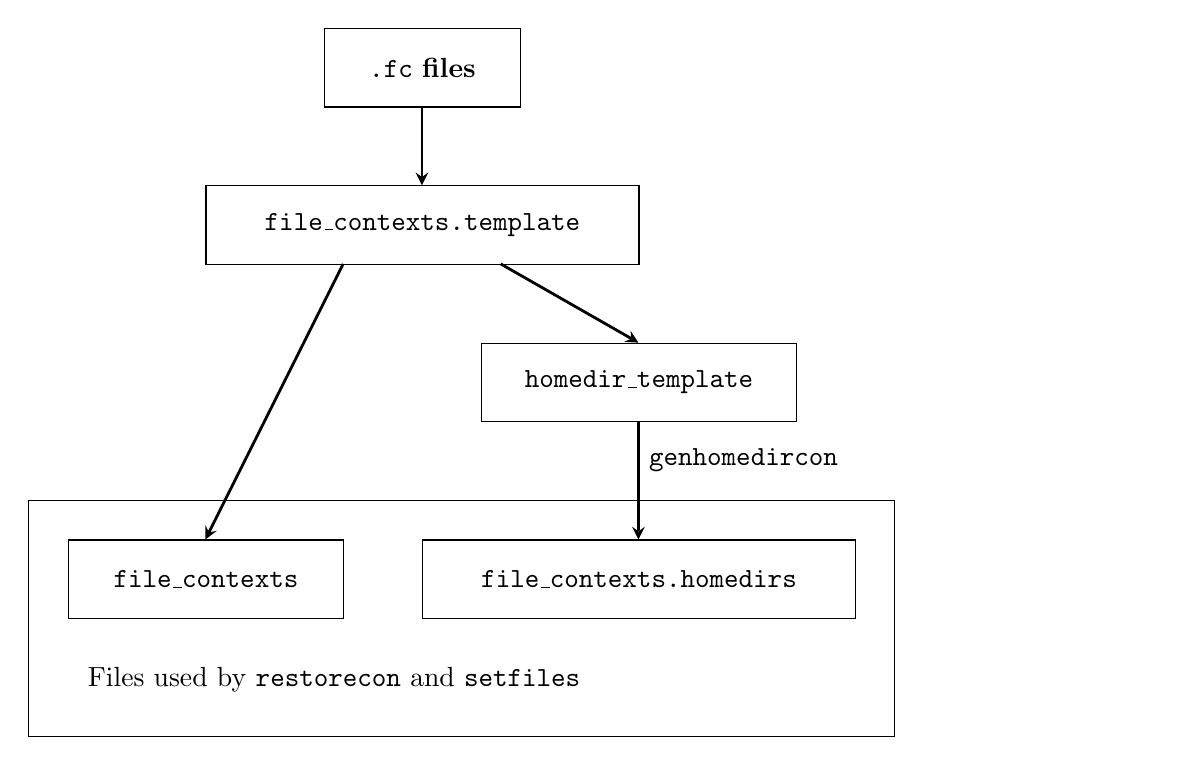
\begin{tikzpicture}
    \usetikzlibrary{calc}
    \tikzstyle{arrow} = [->,>=stealth, line width=1pt]
    \tikzstyle{darrow} = [<->,>=stealth, line width=1pt]
    \tikzstyle{rec} = [rectangle, draw=black, align=center, text width=3.5cm,
        minimum height=1cm, minimum width=4cm, fill=white]

    \draw (0,-6.5) rectangle (11,-9.5);
    %\draw[step=1cm,gray,very thin] (0,0) grid (11,-8);

    \node(fcfiles) [rec, text width=2cm, minimum width=2.5cm]
        at (3.75,-0.5) [anchor=north west]
        {\textbf{\texttt{.fc} files}};

    \node(fctemp) [rec, text width=5cm, minimum width=5.5cm]
        at (2.25,-2.5) [anchor=north west]
        {\textbf{\texttt{file\_contexts.template}}};

    \node(fc) [rec, text width=3cm, minimum width=3.5cm]
        at (0.5,-7) [anchor=north west]
        {\textbf{\texttt{file\_contexts}}};

    \node(hdtemp) [rec, text width=3.5cm, minimum width=4cm]
        at (5.75,-4.5) [anchor=north west]
        {\textbf{\texttt{homedir\_template}}};

    \node(fchd) [rec, text width=5cm, minimum width=5.5cm]
        at (5,-7) [anchor=north west]
        {\textbf{\texttt{file\_contexts.homedirs}}};

    \node(text) [text width=13.5cm, minimum width=14cm]
        at (0.5,-8.5) [anchor=north west]
        {Files used by \texttt{restorecon} and \texttt{setfiles}};

    \draw[arrow] (5,-1.5) -- (5,-2.5);
    \draw[arrow] (4,-3.5) -- (2.25,-7);
    \draw[arrow] (6,-3.5) -- (7.75,-4.5);
    \draw[arrow] (7.75,-5.5) -- node[pos=0.33,right] {\texttt{genhomedircon}}
        (7.75,-7);
\end{tikzpicture}

    \caption{File Context Files}
\end{figure}

These files are created when building policy, see figure \ref{fig:filecontexts}.
All \texttt{.fc} files from base policy and from policy modules are used to
build the \texttt{file\_contexts.template} file. This file may contain rules
that have special keywords inside their path, such as \texttt{HOME\_ROOT},
\texttt{HOME\_DIR}, or \texttt{USER}. All rules without special keywords are
used to build the \texttt{file\_contexts} file used directly by utilities such
as restorecon or setfiles.

Rules with special keywords are used to build the \texttt{homedir\_template}
file. These rules are asssociated with user home directories and need to be
expanded for individual users using the genhomedircon utility. For example the
following \texttt{homedir\_template} entry:
\begin{lstlisting}
HOME_DIR/\.ssh(/.*)?        system_u:object_r:ssh_home_t:s0
\end{lstlisting}
would be expanded to the following rules:
\begin{lstlisting}
/home/[^/]*/\.ssh(/.*)?     system_u:object_r:ssh_home_t:s0
/root/\.ssh(/.*)?           system_u:object_r:ssh_home_t:s0
\end{lstlisting}
Expanded rules are then stored in the \texttt{file\_contexts.homedirs} file and
used by restorecon and setfiles utilities \cite[pp.~134--140]{tsn}.

\subsection{Changing File Context Configuration Files}
The \texttt{file\_contexts.local} file can be changed using the \texttt{semanage
fcontext} command \cite{selinuxguide}. For example:
\begin{lstlisting}
# semanage fcontext -a -t samba_share_t /etc/myfile
# semanage fcontext -l -C
SELinux fcontext    type        Context
/etc/myfile         all files   system_u:object_r:samba_share_t:s0
\end{lstlisting}
In this example, new file contexts entry was added. The rule states that file
\texttt{/etc/myfile} should obtain context
\texttt{system\_u:object\_r:samba\_share\_t:s0}.

% ------------------------------------------------------------------------------
% TOPIC: Auditing
% ----------------------------------------
% STATUS: 4
% 2.16 AUDITING SELINUX EVENTS                                          Y
%     2.16.1 AVC Audit Events                                           Y
%     2.16.2 General SELinux Audit Events                               Y
\section{Auditing Security Events}

The \emph{Linux Audit system} provides an auditing system for tracking
security-relevant system events. It is used to track file access, monitor system
calls, record commands run by user, record failed login attempts and others
\cite{secguide}. The Linux Audit system does not provide additional security by
itself, it can be only used to discover security violations.

The Linux Audit system consists of kernel and userspace part. Kernel filters
events and sends them to the \emph{audit daemon}. Audit daemon then writes the
received events to a~log file. There are several userspace tools used for
interacting with the audit system and for working with the log file.

\subsection{Auditing SELinux Denials}

In Fedora and RHEL, SELinux uses the Linux Audit system to log security events.
When a~process tries to perform operation without the permissions, an
\emph{Access Vector Cache} (AVC) denial message is logged using the audit daemon
\cite{selinuxguide}. This message can be then processed by tools such as
setroubleshoot or audit2allow.

Every AVC message contains information about source context (the context of the
process), object class (for example file), and target context (the context of
the object). For example, when a~process \texttt{httpd} running in context
\texttt{unconfined\_u:system\_r:httpd\_t:s0} is trying to perform the
\texttt{getattr} operation on file \texttt{/var/www/html/file1} with context
\texttt{system\_u:object\_r:samba\_share\_t:s0} and fails, the following AVC
message is generated:

\begin{lstlisting}
type=AVC msg=audit(1223024155.684:49): avc:  denied  { getattr }
for pid=2000 comm="httpd" path="/var/www/html/file1" dev=dm-0
ino=399185 scontext=unconfined_u:system_r:httpd_t:s0
tcontext=system_u:object_r:samba_share_t:s0 tclass=file
\end{lstlisting}

% ------------------------------------------------------------------------------
% TOPIC: Troubleshooting
% ----------------------------------------
% STATUS: 4
% 11. Troubleshooting
%     11.1. What Happens when Access is Denied
%     11.2. Top Three Causes of Problems
%         11.2.1. Labeling Problems
%         11.2.2. How are Confined Services Running?
%         11.2.3. Evolving Rules and Broken Applications
%     11.3. Fixing Problems
%         11.3.1. Linux Permissions
%         11.3.2. Possible Causes of Silent Denials
%         11.3.3. Manual Pages for Services
%         11.3.4. Permissive Domains
%         11.3.5. Searching For and Viewing Denials
%         11.3.6. Raw Audit Messages
%         11.3.7. sealert Messages
%         11.3.8. Allowing Access: audit2allow
\section{Troubleshooting SELinux}
% SELinux denial - what happens, logs
% auditd
% setroubleshootd
% labeling problems
% services running with wrong context
% ports
% linux perms
% silent denials - dontaudit rules
% permissive domains
% viewing denials
% sealert
% audit2allow

When SELinux denies access that is requested by a~process, the process may fail
to function normally and reports error or crashes. Determining if the failure is
related to SELinux is done by switching whole SELinux or just one domain into
permissive mode. For example, for debugging \texttt{httpd} it is advised to set
the \texttt{httpd\_t} domain into permissive mode:
\begin{lstlisting}
# semanage permissive -a httpd_t
\end{lstlisting}
SELinux denials caused by the \texttt{httpd\_t} domain would still be logged but
not enforced.

On Fedora and RHEL, SELinux denials are analyzed by the \texttt{setroubleshootd}
daemon that provides suggestions for resolving the problem using various
plugins. Majority of problems are caused by missing \texttt{allow} rules in
policy. To add missing rules, the audit2allow utility is used. However, not
every problem requires new policy rules, some issues may require relabeling of
objects using restorecon or semanage.

% ------------------------------------------------------------------------------
\section{The audit2allow Utility}
% STATUS: 4
\label{audit2allow}
The audit2allow is a~userspace tool that scans the AVC messages and generates
SELinux policy snippets based on them.

\subsection{Purpose of audit2allow}
% STATUS: 4
The audit2allow utility is designed both for system administrators and SELinux
policy developers. System administrators use audit2allow to analyze SELinux
denials and to create new policy modules. When suitable, the audit2allow utility
suggests other options to resolve denials, such as turning on a~boolean (see
section \ref{booleans}).

Policy developers use audit2allow to create basis for new policy modules for
their products. When writing policy for their program, they can run the
programs test suite in permissive mode, collect AVC denials, create policy
module, and then manually finish the policy module. Policy developers can use
the \texttt{-{}-reference} option to generate policy using predefined macros.

\subsection{Basic Mode of Operation}
% STATUS: 4
In default mode, audit2allow scans AVC denial messages and generates policy
rules which allow operations that were denied. For example, when the
\texttt{httpd} process tries to perform the \texttt{getattr} operation on the
\texttt{/var/www/html/file1} file, the following AVC message is generated:
\begin{lstlisting}[escapechar=\%]
type=%\textbf{AVC}% msg=audit(1223024155.684:49): avc:  denied  { %\textbf{getattr}% }
for pid=2000 comm="%\textbf{httpd}%" path="%\textbf{/var/www/html/file1}%" dev=dm-0
ino=399185 scontext=%\textbf{unconfined\_u:system\_r:httpd\_t:s0}%
tcontext=%\textbf{system\_u:object\_r:samba\_share\_t:s0}% tclass=%\textbf{file}%
\end{lstlisting}
The audit2allow utility would generate the following policy rule:
\begin{lstlisting}
allow httpd_t samba_share_t:file getattr;
\end{lstlisting}
The audit2allow utility is able process multiple AVC denial messages, deal with
duplicates, and output all rules based on fields in AVC denial messages.

\subsection{Command-Line Options}
% STATUS: 4
The audit2allow utility is able to read AVC messages from stdin, dmesg, audit
log, or arbitrary file (see \texttt{-{}-dmesg}, \texttt{-{}-all}, and
\texttt{-{}-input} options). There is \texttt{-{}-boot} option which loads only
messages generated since last boot and \texttt{-{}-lastreload} option which
loads only messages since last SELinux policy reload.

The audit2allow utility can output the policy rules directly to stdout or file,
or create a~policy module which can be loaded directly into the policy (see
\texttt{-{}-module}, \texttt{-M}, and \texttt{-{}-output} options).

The audit2allow utility is using currently loaded policy (or any other policy
specified with the \texttt{-{}-policy} option) to get more information about the
denials. For example, audit2allow suggests turning on a~boolean that would allow
the denied operations.

When run with the \texttt{-{}-reference} option, audit2allow tries to match the
denials against defined interfaces. Example of audit2allow output without the
\texttt{-{}-reference} option:
\begin{lstlisting}
#============= httpd_t ==============
allow httpd_t samba_share_t:file getattr;
\end{lstlisting}
Example of audit2allow output with the \texttt{-{}-reference} option:
\begin{lstlisting}
require {
	type httpd_t;
}

#============= httpd_t ==============
samba_read_share_files(httpd_t)
\end{lstlisting}
The audit2allow found an interface which contained the same allow rule.
Interfaces create more readable code but can contain more rules that are
necessary.

The \texttt{-{}-why} option does not output any policy rules but provides a~text
description of why the access was denied. Example of \texttt{audit2allow
-{}-why} output:
\begin{lstlisting}
type=AVC msg=audit(1223024155.684:49): avc: denied { getattr }
for pid=2000 comm="httpd" path="/var/www/html/file1" dev=dm-0
ino=399185 scontext=unconfined_u:system_r:httpd_t:s0
tcontext=system_u:object_r:samba_share_t:s0 tclass=file

    Was caused by:
        Missing type enforcement (TE) allow rule.

        You can use audit2allow to generate a~loadable module
        to allow this access.
\end{lstlisting}

The \texttt{-{}-dontaudit} option generates \texttt{dontaudit} rules instead of
\texttt{allow} rules (see section~\ref{avrules}).

\subsection{How Does audit2allow Work}
% STATUS: 4
The audit2allow first collects audit messages from various sources. Messages are
stored based on their type and then parsed. Every AVC denial message is analyzed
together with binary policy file to find out the reason of denial.

From AVC denial messages, source contexts, target contexts, object classes, and
permissions are extracted and converted into \emph{access vector sets}. Each
access vector in the set contains unique combination of source context, target
context, and object class. Permissions from multiple AVC messages are merged
into one access vector set. Example of an access vector set:
\begin{lstlisting}[language=Python]
{
  {
    src: 'unconfined_u:system_r:httpd_t:s0',
    tgt: 'system_u:object_r:samba_share_t:s0',
    cls: 'file', perms: [ 'getattr', 'open' ]
  },
  {
    src: 'unconfined_u:system_r:httpd_t:s0',
    tgt: 'system_u:object_r:sssd_conf_t:s0',
    cls: 'file', perms: [ 'getattr' ]
  }
}
\end{lstlisting}

Each access vector is then converted into an allow rule. All rules are printed
to the output. Example:
\begin{lstlisting}
allow httpd_t samba_share_t:file { getattr open };
allow httpd_t sssd_conf_t:file getattr;
\end{lstlisting}
The \texttt{module} and \texttt{require} statements (see section \ref{modules})
may be optionally written to the output. Various other information is stored
during processing. The audit2allow prints comments with helpful messages.

\subsection{Implementation of audit2allow}
% STATUS: 4
\label{implementation}
The audit2allow utility is part of SELinux userspace. It is written mostly in
Python with several parts written in C. It uses sepolgen and sepolicy Python
packages and libselinux and libsepol libraries.

Main script, \texttt{audit2allow}, parses command-line options, retrieves audit
messages, and prints the output.  Main logic of converting AVC denial messages
to access vector rules is implemented in package sepolgen.

The sepolgen package contains the following modules:
\begin{description}
    \item [\texttt{audit.py}] Defines classes for various audit messages,
        contains audit message parser.
    \item [\texttt{access.py}] Defines access vectors and access vector sets.
    \item [\texttt{policygen.py}] Creates policy rules based on access vectors.
    \item [\texttt{refpolicy.py}] Contains classes that represent the policy
        statements.
    \item [\texttt{output.py}] Outputs the generated rules.
    \item [Other modules] There are several other modules which are either not
        significant (e.g. the \texttt{utils.py} module) or used only for
        generating policy using interfaces (e.g. the \texttt{interfaces.py}
        package).
\end{description}

\subsubsection{The audit2allow Script}
% STATUS: 4
% parse options
% load policy
    % init the audit2why C module
% read input
    % creates audit parser
    % reads messages
    % feeds them to the parser
% process input
    % filters messages if neccessary
    % converts messages to access vectors
% output
    % output audit2why if selected
    % creates policy generator
    % sets options to the generator
    % adds AVs to the generator
    % writes the output

The main script does the following steps:
\begin{enumerate}
    \item Parse command-line arguments and check potential conflicts.
    \item Read audit messages. Create \texttt{AuditParser} instance and feed it
        the messages.
    \item Filter the messages (if specified by the \texttt{-{}-type} option) and
        convert them to access vectors.
    \item Create and setup a~\texttt{PolicyGenerator} instance, feed it the
        access vectors, and convert them to policy rules.
    \item Write the output.
\end{enumerate}

\subsubsection{The audit.py Module}
% STATUS: 4
% convenience functions
% AuditMessage class
    % base class for all messages
% InvalidMessage class
% PathMessage class
% PolicyLoadMessage class
% DaemonStartMessage class
% ComputeSidMessage class
% AVCMessage class
    % from_split_string
    % analyze
% AuditParser class
    % parse_file, parse_string
    % to_role, to_access
% AVCTypeFilter
% ComputeSidTypeFilter

The \texttt{audit.py} module is used for parsing audit messages. It is not a
general purpose audit parsing library, it is meant to parse mainly AVC messages
and policy load messages.

The \texttt{AuditParser} class reads strings and creates objects of appropriate
type for each message. The \texttt{AuditMessage} class is the base class for all
message types. The \texttt{AVCMessage} class represents AVC denials and is used
for generating access vectors.

After parsing of AVC message, the denial is analyzed in \texttt{audit2why.c}
module (from libselinux library). The \texttt{audit2why.c} module tries to find
out the reason of the denial by analyzing the policy. The module is written in C
and uses the libsepol library.

Each message is then converted to an access vector from the \texttt{access}
module. AVC denial messages can be filtered using regular expressions via the
\texttt{AVCTypeFilter} class. Only messages that match the regular expression
are processed.

Policy load messages are important for the \texttt{-{}-lastreload} command-line
option. The \texttt{AuditParser} then processes only messages after last policy
load message.

\subsubsection{The access.py Module}
% STATUS: 4
% AccessVector
    % basic representation of access
    % single source and target type, single object class, set of permissions
% AccessVectorSet
    % used for storing AVs
    % AVs with same source and target type and class are merged
    % add() adds AV to the set
% RoleTypeSet

The \texttt{access.py} module defines the \texttt{AccessVector} and
\texttt{AccessVectorSet} classes. Access vector is a~basic representation of an
access in SELinux. It contains single source and target type, single object
class, and a~set of permissions. Every AVC denial message can be converted into
an access vector. For example this AVC denial message:
\begin{lstlisting}[escapechar=\%]
type=AVC msg=audit(1223024155.684:49): avc:  denied  { %\textbf{getattr}% }
for pid=2000 comm="httpd" path="/var/www/html/file1" dev=dm-0
ino=399185 scontext=%\textbf{unconfined\_u:system\_r:httpd\_t:s0}%
tcontext=%\textbf{system\_u:object\_r:samba\_share\_t:s0}% tclass=%\textbf{file}%
\end{lstlisting}
would be converted into the following access vector:
\begin{lstlisting}[language=Python]
{
    source_context: 'unconfined_u:system_r:httpd_t:s0',
    target_context: 'system_u:object_r:samba_share_t:s0',
    object_class: 'file',
    permissions: [ 'getattr' ]
}
\end{lstlisting}

Multiple access vectors are aggregated in access vector sets. Access vectors
that share the same source and target type and object class are merged together
so that there are no duplicates. For example, if we add the following access
vector:
\begin{lstlisting}[language=Python]
{
    source_context: 'unconfined_u:system_r:httpd_t:s0',
    target_context: 'system_u:object_r:samba_share_t:s0',
    object_class: 'file',
    permissions: [ 'open', 'read' ]
}
\end{lstlisting}
to the access vector above, they would be merged into the following access
vector (they share source and target context and object class):
\begin{lstlisting}[language=Python]
{
    source_context: 'unconfined_u:system_r:httpd_t:s0',
    target_context: 'system_u:object_r:samba_share_t:s0',
    object_class: 'file',
    permissions: [ 'getattr', 'open', 'read' ]
}
\end{lstlisting}

Access vector sets serve as a~basis for generating policy access vector rules
in the \texttt{policygen.py} module.

\subsubsection{The policygen.py Module}
% STATUS: 4
% PolicyGenerator
    % generates policy module from access vectors
    % has several options
    % set_gen_refpol()
    % set_gen_requires()
    % set_gen_explain()
    % set_gen_dontaudit()
    % add_access()
% explain_access()
% call_interface()
% InterfaceGenerator
% gen_requires()
The \texttt{policygen.py} module defines the \texttt{PolicyGenerator} class that
generates policy module from access vectors. \texttt{PolicyGenerator} converts
access vector set into SELinux policy statements. For example, this access
vector:
\begin{lstlisting}[language=Python]
{
    source_context: 'unconfined_u:system_r:httpd_t:s0',
    target_context: 'system_u:object_r:samba_share_t:s0',
    object_class: 'file',
    permissions: [ 'getattr', 'open', 'read' ]
}
\end{lstlisting}
would be converted into the following policy statement:
\begin{lstlisting}
allow httpd_t samba_share_t:file { getattr open read };
\end{lstlisting}

\texttt{PolicyGenerator} uses objects from the \texttt{refpolicy.py} module
to represent policy statements. \texttt{PolicyGenerator} provides several
configuration methods:
\begin{description}
    \item [\texttt{set\_gen\_refpol()}] Turn on interface generation.
    \item [\texttt{set\_gen\_requires()}] Generate \texttt{require} statements
        that are neccessary for creating a~standalone policy module (see section
        \ref{modules}).
    \item [\texttt{set\_gen\_explain()}] Add comments explaining why were the
        policy statements generated.
    \item [\texttt{set\_gen\_dontaudit()}] Generate \texttt{dontaudit} rules
        instead of \texttt{allow} rules (see section \ref{avrules}).
\end{description}
The output of \texttt{PolicyGenerator} is a~tree-like structure containing
generated policy statements. The \texttt{output.py} module then just prints out
every statement.

\subsubsection{The refpolicy.py Module}
% STATUS: 4
% PolicyBase
% Node
% Leaf
% walktree, walknode, list_to_space_str, list_to_comma_str
% IdSet
% SecurityContext
% ObjectClass
% TypeAttribute, RoleAttribute
% Role, Type, TypeAlias
% Attribute, AttributeRole
% AVRule
% TypeRule, TypeBound
% RoleAllow, RoleType
% ModuleDeclaration
% Conditional, Bool
% InitialSid, GenfsCon, FilesystemUse
% PortCon, NodeCon, NetifCon, PirqCon, IomemCon, IoportCon
% print_tree
% Headers
% Module
% Interface, TunablePolicy, Template, IfDef, InterfaceCall, OptionalPolicy,
% SupportMacros, Require
% ObjPermSet, ClassMap
% Comment
This module contains classes that represent SELinux policy statements. The
\texttt{Node} and \texttt{Leaf} classes are base classes for all policy
statements. Every statement is either a~node that is a~parent of other
statements (for example the \texttt{Module} class), or a~leaf (for example the
\texttt{AVRule} class). The \texttt{refpolicy.py} module contains functions for
traversing trees made out of nodes and leaves. These functions are used when
printing statements in the \texttt{output.py} module.

The \texttt{IdSet} class represents set of arbitrary identifiers and is used by
many statements for storing permissions and other sets. The
\texttt{SecurityContext} class represents an SELinux security context. Classes
such as \texttt{TypeAttribute}, \texttt{RoleAttribute}, \texttt{Role},
\texttt{Type}, and others represent policy statements as described in section
\ref{policy} and are used mainly for interface generation.

For basic operation mode, the following classes are used: \texttt{AVRule},
\texttt{ModuleDeclaration}, \texttt{Module}, and \texttt{Require}. The
\texttt{AVRule} class contains the following attributes:
\begin{description}
    \item [\texttt{src\_types}] \texttt{IdSet()} of source types.
    \item [\texttt{tgt\_types}] \texttt{IdSet()} of target types.
    \item [\texttt{obj\_classes}] \texttt{IdSet()} of object classes.
    \item [\texttt{perms}] \texttt{IdSet()} of permissions.
    \item [\texttt{rule\_type}] One of the following: \texttt{ALLOW},
        \texttt{DONTAUDIT}, \texttt{AUDITALLOW}, or \texttt{NEVERALLOW}.
\end{description}
Class \texttt{Module} serves only as a~node that is parent to all statements
inside a~module. Class \texttt{ModuleDeclaration} represents the
\texttt{module} statement and is generated with the \texttt{-{}-module} option.
Class \texttt{Require} represent the \texttt{require} statement inside policy
modules and is generated with either \texttt{-{}-module} or \texttt{-{}-require}
options.

% ----------------------------------------
% THE SELINUX NOTEBOOK
% 2.11 COMPUTING ACCESS DECISIONS                                       ?
% 2.17 POLYINSTANTIATION SUPPORT                                        N
%     2.17.1 Polyinstantiated Objects                                   N
%     2.17.2 Polyinstantiation support in PAM                           N
%         2.17.2.1 namespace.conf Configuration File                    N
%         2.17.2.2 Example Configurations                               N
%     2.17.3 Polyinstantiation support in X-Windows                     N
%     2.17.4 Polyinstantiation support in the Reference Policy          N
% 2.18 PAM LOGIN PROCESS                                                N
% 2.20 LIBSELINUX LIBRARY                                               N
% 4.12 CONSTRAINT STATEMENTS                                            ?
%     4.12.1 constrain                                                  ?
%     4.12.2 validatetrans                                              ?
%     4.12.3 mlsconstrain                                               ?
%     4.12.4 mlsvalidatetrans                                           ?
% 4.13 MLS STATEMENTS                                                   N
%     4.13.1 sensitivity                                                N
%     4.13.2 dominance                                                  N
%     4.13.3 category                                                   N
%     4.13.4 level                                                      N
%     4.13.5 range_transition                                           N
%         4.13.5.1 MLS range Definition                                 N
%     4.13.6 mlsconstrain                                               N
%     4.13.7 mlsvalidatetrans                                           N
% 4.14 SECURITY ID (SID) STATEMENT                                      N
%     4.14.1 sid                                                        N
%     4.14.2 sid context                                                N
% 4.15 FILE SYSTEM LABELING STATEMENTS                                  N
%     4.15.1 fs_use_xattr                                               N
%     4.15.2 fs_use_task                                                N
%     4.15.3 fs_use_trans                                               N
%     4.15.4 genfscon                                                   N
% 4.18 XEN STATEMENTS                                                   N
%     4.18.1 iomemcon                                                   N
%     4.18.2 ioportcon                                                  N
%     4.18.3 pcidevicecon                                               N
%     4.18.4 pirqcon                                                    N
%     1.5. Additional Resources
% SELINUX GUIDE
% 3. Targeted Policy
%     3.1. Confined Processes
%     3.2. Unconfined Processes
%     3.3. Confined and Unconfined Users
%         3.3.1. The sudo Transition and SELinux Roles
% 4. Working with SELinux
%     4.1. SELinux Packages
%     4.2. Which Log File is Used
%     4.3. Main Configuration File
%     4.4. Permanent Changes in SELinux States and Modes
%         4.4.1. Enabling SELinux
%         4.4.2. Disabling SELinux
%     4.5. Changing SELinux Modes at Boot Time
%     4.11. Information Gathering Tools
%     4.12. Prioritizing and Disabling SELinux Policy Modules
%     4.15. Disabling ptrace()
%     4.16. Thumbnail Protection
% 5. The sepolicy Suite
%     5.1. The sepolicy Python Bindings
%     5.2. Generating SELinux Policy Modules: sepolicy generate
%     5.3. Understanding Domain Transitions: sepolicy transition
%     5.4. Generating Manual Pages: sepolicy manpage
% 6. Confining Users
%     6.1. Linux and SELinux User Mappings
%     6.2. Confining New Linux Users: useradd
%     6.3. Confining Existing Linux Users: semanage login
%     6.4. Changing the Default Mapping
%     6.5. xguest: Kiosk Mode
%     6.6. Booleans for Users Executing Applications
% 7. Securing Programs Using Sandbox
%     7.1. Running an Application Using Sandbox
% 8. sVirt
%     8.1. Security and Virtualization
%     8.2. sVirt Labeling
% 9. Secure Linux Containers
% 10. SELinux systemd Access Control
%     10.1. SELinux Access Permissions for Services
%     10.2. SELinux and journald
% 12. Further Information
%     12.1. Contributors
%     12.2. Other Resources

% ==============================================================================
\chapter{Analysis}
% STATUS: 4
Two general areas for improvement to audit2allow were identified:
\begin{enumerate}
    \item Changing label of an object instead of creating new policy rules. This
        includes checking of mislabeled files, labeling network ports, nodes,
        and interfaces.
    \item Support for new SELinux policy statements such as extended permission
        access vector rules.
\end{enumerate}

% ------------------------------------------------------------------------------
\section{Extended Permission Access Vector Rules}
% STATUS: 4
Since policy version 30, SELinux policy supports extended permission access
vector rules (see section \ref{extavrules}). Usage of extended permission AV
rules introduces situations when audit2allow is not able to detect the true
cause of denial. As a~result, when using extended permission AV rules,
audit2allow may suggest rules that do not solve the denial.

\subsection{AVC Denials Caused by Extended Permission AV Rules}
% STATUS: 4
Suppose there are following rules present in the policy:
\begin{lstlisting}
allow src_t tgt_t : tcp_socket ioctl;
allowxperm src_t tgt_t : tcp_socket ioctl 0x42;
\end{lstlisting}
When a~process tries to call \texttt{ioctl(0x1234, ...)}, the operation would be
denied, because only syscall \texttt{ioctl(0x42, ...)} is allowed. The following
AVC denial message would be generated:
\begin{lstlisting}[escapechar=\%]
type=AVC msg=audit(1515017775.689:1722): avc:  denied  { ioctl } for
pid=14587 comm="test" dev="dm-0" ino=8390105 %\textbf{ioctlcmd=0x1234}%
scontext=unconfined_u:unconfined_r:src_t:s0-s0:c0.c1023
tcontext=unconfined_u:object_r:tgt_t:s0 tclass=tcp_socket permissive=0
\end{lstlisting}
The \texttt{ioctlcmd} field contains the first parameter of the ioctl syscall
that was denied. This value can be used to construct an \texttt{allowxperm} rule
to allow this operation.

When used for troubleshooting this AVC denial, audit2allow produces the
following output:
\begin{lstlisting}
#============= src_t ==============

#!!!! This avc is allowed in the current policy
allow src_t tgt_t:tcp_socket ioctl;
\end{lstlisting}
which is not helpful. Users are expected to know about extended permissions to 
assume that the allow rule was overridden.

\subsection{Generating Extended Permission AV Rules in audit2allow}
% STATUS: 4
% example 1: no rule
% example 2: both allow and allow rule
The audit2allow does have all the information to generate extended permission AV
rules. There are two situations that may arise when using extended permission AV
rules:
\begin{itemize}
    \item There is neither \texttt{allow} nor \texttt{allowxperm} rule in the
        policy. The audit2allow utility has two options: either generate only
        allow rule (current behaviour) or generate \texttt{allow} and
        \texttt{allowxperm} rules. Generating \texttt{allowxperm} rules is more
        secure and provides more granular access control. However, for many
        processes that use lot of different ioctl calls it may be inefficient.
        Generating the \texttt{allowxperm} rules automatically also changes the
        default output of audit2allow and breaks lot of integration tests
        written using the audit2allow utility.
    \item There is both \texttt{allow} and \texttt{allowxperm} rule in the
        policy. This means that the specific ioctl parameter is not allowed. In
        this case \texttt{allowxperm} rule should be generated.
\end{itemize}

It is not possible to distinguish these two sitautions by analyzing the AVC
denial itself, because both denials contain the \texttt{ioctlcmd} field. The
audit2allow utility would need to analyze the binary policy. The audit2allow
utility may rather generate extended permission AV rules in all cases (stricter,
more secure solution) or only when requested by user (for example using
command-line option, less secure solution, does not break backward
compatibility).

In case of using command-line option, there is still a~risk, that the user does
not know that he or she should be using that option. Consider the following
example:
\begin{lstlisting}
#============= src_t ==============

#!!!! This avc is allowed in the current policy
allow src_t tgt_t:tcp_socket ioctl;
\end{lstlisting}
In this example, it is not clear that the denial is caused by extended
permission AV rule. In situations when the denial would be allowed according to
the binary policy (there is an \texttt{allow} rule) and the AVC denial message
contains the \texttt{ioctlcmd} field, the user should be warned about extended
permission AV rules. For example:
\begin{lstlisting}
#============= src_t ==============

#!!!! This avc is allowed in the current policy
#!!!! This av rule may have been overriden by extended permission av rule
allow src_t tgt_t:tcp_socket ioctl;
\end{lstlisting}
Support for extended permissions was implemented as a~part of this thesis, see
section \ref{xpermsimp}.

% ------------------------------------------------------------------------------
\section{Mislabeled Files}
% STATUS: 4
\label{mislabeled}
SELinux relies on files having correct label. Sometimes, when files get
mislabeled, processes cannot access these files and causes AVC denials. When
used for troubleshooting, audit2allow suggests adding new rules to the policy
instead of changing label of the file.

\subsection{AVC Denial Messages Caused by Mislabeled Files}
% STATUS: 4
When a~process is trying to access file that is mislabeled, the operation is
usually denied (unless the process has access also to the incorrect label). For
example, when user moves content from \texttt{/root} directory to the
\texttt{/var/www/html/} directory, files retain their original label:
\begin{lstlisting}
$ ls /var/www/html
unconfined_u:object_r:httpd_sys_content_t:s0 index.html
       unconfined_u:object_r:admin_home_t:s0 my_file.html
\end{lstlisting}
File \texttt{index.html} has correct label, but file \texttt{my\_file.html} has
an incorrect label. The \texttt{httpd} process cannot access files labeled
\texttt{admin\_home\_t}, because there are no allow rules in the policy for this
operation:
\begin{lstlisting}
$ sesearch -A -s httpd_t -t admin_home_t -c file -p read
(nothing)
\end{lstlisting}

As a~result, when trying to view \texttt{my\_file.html}, similar AVC denial
message is generated:
\begin{lstlisting}
type=AVC msg=audit(1226270358.848:238): avc:  denied  { read }
for  pid=13349 comm="httpd" ino=8390105 name="my_file.html"
dev=dm-0 ino=218171 scontext=system_u:system_r:httpd_t:s0
tcontext=system_u:object_r:admin_home_t:s0 tclass=file
\end{lstlisting}
In this case, there is the \texttt{ino} field, which contains inode number
associated with the denial, and the \texttt{name} field, which contains the name
of the file (but not the full path). In cases of \texttt{getattr} denial, the
\texttt{path} field is present.

\subsection{Solving Problems With Mislabeled Files}
The restorecon utility uses file contexts files to get default security contexts
of files (see section \ref{filecontexts}). For example, when file
\texttt{/var/www/html/my\_file.html} is mislabeled, the denial should be fixed
by running restorecon on the file:
\begin{lstlisting}
# restorecon -v /var/www/html/my_file.html
Relabeled /var/www/html/my_file.html from unconfined_u:object_r:
admin_home_t:s0 to unconfined_u:object_r:httpd_sys_content_t:s0
\end{lstlisting}

When using audit2allow, the following rules are generated:
\begin{lstlisting}
allow httpd_t admin_home_t:file getattr;
\end{lstlisting}
This means that the \texttt{httpd} process would gain access to all root's
files. This solution is not secure because it is adding unnecessary rules to the
policy and it does not solve the real problem.

\subsection{Improving audit2allow}
% STATUS: 4
The audit2allow utility should detect when the AVC message is caused by
mislabeled file and suggest solution using the restorecon utility.

There are three fields in the AVC message that can be used to detect if the file
was mislabeled: \texttt{path}, \texttt{name} and \texttt{inode}. When the
\texttt{path} field is present, audit2allow can run \texttt{matchpathcon} to get
the default context of the file and compare it with actual file context.

In many cases, the \texttt{path} field is not present, only inode number and
name of the file (without full path). In this case it is difficult to find the
full path of the file. Ryan Hallisey created solution \cite{restoreconpullreq}
that is using \texttt{locate} utility to get all files matching the name and
then stat these files to get the inode number. This solution is only partial, it
does not work on files that are not indexed in the database created by
\texttt{updatedb}.

% ------------------------------------------------------------------------------
\section{Labeling Network Ports, Nodes, and Interfaces}
\label{networkobjects}
SELinux policy supports labeling of TCP and UDP ports, network nodes
(represented by IP addresses and subnet masks), and network interfaces (e.g.
\texttt{eth0}).

\subsection{Network Ports}
% STATUS: 4
SELinux can enforce binding to system ports. For example, in Fedora 27, there
are several hundred \texttt{portcon} rules that label TCP and UDP ports.
Example:
\begin{lstlisting}
$ seinfo --portcon

Portcon: 615
   portcon tcp 1-511 system_u:object_r:reserved_port_t:s0
   portcon tcp 7 system_u:object_r:echo_port_t:s0
   portcon tcp 21 system_u:object_r:ftp_port_t:s0
   portcon tcp 22 system_u:object_r:ssh_port_t:s0
   portcon tcp 53 system_u:object_r:dns_port_t:s0
   portcon tcp 80 system_u:object_r:http_port_t:s0
   portcon udp 1-511 system_u:object_r:reserved_port_t:s0
   portcon udp 1 system_u:object_r:inetd_child_port_t:s0
   portcon udp 7 system_u:object_r:echo_port_t:s0
   portcon udp 53 system_u:object_r:dns_port_t:s0
   portcon udp 67 system_u:object_r:dhcpd_port_t:s0
   ...
\end{lstlisting}
Portcon rules can overlap, for example TCP port number 80 is labeled
\texttt{http\_port\_t} but also \texttt{reserved\_port\_t} because it is in range
1--511. Every port has either domain-specific label or one of the following
labels (based on range):

\begin{tabular}{l l}
    1--511 & \texttt{reserved\_port\_t} \\
    512--1023 & \texttt{hi\_reserved\_port\_t} \\
    1024--32767 & \texttt{unreserved\_port\_t} \\
    32768--61000 & \texttt{ephemeral\_port\_t} \\
    61001--65535 & \texttt{unreserved\_port\_t} \\
\end{tabular}

When a~process tries to bind to a~port and it is denied by SELinux, AVC denial
message is generated. For example:
\begin{lstlisting}[escapechar=\%]
type=AVC msg=audit(1516026512.648:4191): avc:  denied  { name_bind } for
pid=6116 comm="test" %\textbf{src=43}% scontext=unconfined_u:unconfined_r:my_app_t:s0
tcontext=system_u:object_r:reserved_port_t:s0
tclass=tcp_socket permissive=0
\end{lstlisting}

Proper way how to allow the process to bind on port number 43 would be to label
this port with a~application-specific context using either a~\texttt{portcon}
rule or the \texttt{semanage port} command. For example:
\begin{lstlisting}
# semanage port --add -t system_u:object_r:my_app_port_t:s0 -p TCP 43
\end{lstlisting}

When used for troubleshooting this denial, the audit2allow utility suggests
adding the following rule to the policy:
\begin{lstlisting}[language=te]
allow my_app_t reserved_port_t:tcp_socket name_bind;
\end{lstlisting}
This rule would allow \texttt{my\_app\_t} access to all reserved ports which is
unneccessary and potentially unsecure.

Ports can be labeled using the \texttt{portcon} rules, but as of policy version
31, these rules are not valid in policy module, only in base policy. So
audit2allow would not be able to generate \texttt{portcon} rules directly.
Another way of labeling ports is via the \texttt{semanage port} command. The
audit2allow should suggest using the \texttt{semanage port} command when
appropriate.

\subsection{Network Nodes}
% STATUS: 4
SELinux is capable of labeling network nodes. For example, there can be rules
that allow process to communicate only on private LAN or even only on local
host. Attempts to violate these rules would then produce AVC denial messages
that contain IP address of the node.

Proper solution would be to modify label of certain subnet of the network, for
example using the \texttt{semanage node} command. AVC denial messages provides
only IP addresses. As IP addresses can change often, labeling single network
node would not be useful. Labeling of network nodes is not used on Fedora and
RHEL. Improving the audit2allow utility to suggest \texttt{semanage node}
commands would not make a~big impact on security.

\subsection{Network Interfaces}
% STATUS: 4
SELinux is capable of labeling network interfaces (such as \texttt{eth0}). In
Fedora and RHEL, labeling of network interfaces is not used. Improving
audit2allow to suggest \texttt{semanage interface} commands would not make a~big
impact on security.

% ==============================================================================
\chapter{Implementation}
% STATUS: 4
From the list of possible improvements to audit2allow, the following
improvements were implemented:
\begin{itemize}
    \item Support for extended permissions. The audit2allow utility can now
        detect denials that may be caused by extended permission AV rules. With
        the \texttt{-{}-xperms} option, audit2allow generates extended AV rules.
    \item Checking mislabeled files. The audit2allow utility now parses the
        \texttt{path} field in AVC denial messages and checks if files have
        default context. When the context in AVC denial message is different
        than the default one, audit2allow produces warning.
\end{itemize}

% ------------------------------------------------------------------------------
\section{Extended Permissions}
% STATUS: 4
\label{xpermsimp}
Main script \texttt{audit2allow} and the \texttt{audit.py}, \texttt{access.py},
\texttt{policygen.py}, \texttt{refpolicy.py} modules were modified to support
extended permissions. Support for extended permission AV rules with the
\texttt{-{}-reference} option was not implemented.

In main script, new command-line option \texttt{-{}-xperms} was added to turn on
generating of the extended permission AV rules. This option turns on extended
permission AV rules generating in \texttt{PoligyGenerator}.

\subsection{Parsing AVC Denial Messages}
% STATUS: 4
Despite extended permissions being a~general concept, AVC denial messages
generated by the Linux Audit system contain operation-specific field
\texttt{ioctlcmd}. In the future, with introduction of new operation to the
extended permissions, the \texttt{audit.py} module will need to be updated.

The \texttt{audit.py} module was extended to parse the \texttt{ioctlcmd} field
in AVC denial messages. The \texttt{ioctlcmd} field is then converted to fit the
general concept of extended permissions and passed to the access vector set. The
following code in the \texttt{AuditParser.to\_access()} method converts
operation-specific fields to generic extended permission dictionary:
\begin{lstlisting}[language=Python]
if avc.ioctlcmd:
    xperm_set = refpolicy.XpermSet()
    xperm_set.add(avc.ioctlcmd)
    xperms = { "ioctl": xperm_set }
\end{lstlisting}

\subsection{Storing Extended Permissions}
% STATUS: 4
AVC denial messages are converted to access vectors (see section
\ref{implementation}). Two messages that contains same source and target context
and object class are merged together. Denials caused by the ioctl system call
produce AVC denial messages containing the \texttt{ioctlcmd} field. These
messages can be treated the same way as any other AVC denial message, but for
generating extended permission AV rules, the \texttt{ioctlcmd} field must be
stored. The \texttt{AccessVector} class was extended to store the
\texttt{ioctlcmd} field and potentionally any other extended permission fields
introduced in the future.

Single access vector may be product of several AVC denial messages that contain
different values in the \texttt{ioctlcmd} field. For the purpose of representing
extended permission values, new class \texttt{XpermSet} was implemented in the
\texttt{refpolicy.py} module. The \texttt{XpermSet} class supports merging of
multiple values. It is likely that in the future new extended permission
operation will be introduced. Access vector must store values for different
operations. For this purpose, \texttt{XpermSet} objects are stored in a
dictionary where the operation is the key, for example:
\begin{lstlisting}
{
    'ioctl': <refpolicy.XpermSet() object>,
    'other_command': <refpolicy.XpermSet() object>,
    'another_command': <refpolicy.XpermSet() object>,
}
\end{lstlisting}

When merging two access vectors, the permissions set are merged using the
\texttt{union()} method. Extended permission dictionary is merged using the
following code from the \texttt{AccessVector.merge()} method:
\begin{lstlisting}[language=Python]
for op in av.xperms:
    if op not in self.xperms:
        self.xperms[op] = refpolicy.XpermSet()
    self.xperms[op].extend(av.xperms[op])
\end{lstlisting}
The \texttt{av} variable contains access vector that is to be merged with
\texttt{self} access vector.

\subsection{Representation of Extended Permission AV Rules}
% STATUS: 4
Extended permission access vector rules are represented by new
\texttt{AVExtRule} class from the \texttt{refpolicy.py} module. This class is
very similar to the \texttt{AVRule} class, but contains attributes specific to
extended permission AV rules. The \texttt{operation} attribute is a~string
identifying the operation, e.g. 'ioctl'. The \texttt{xperms} attribute is an
\texttt{XpermSet} instance. Method \texttt{to\_string()} prints out the rule.
Example of an extended permission AV rule:
\begin{lstlisting}
allowxperm my_app_t my_socket_t : tcp_socket ioctl { 20 30 0x40 50-60 };
\end{lstlisting}

The \texttt{AVExtRule} class is initialized from an access vector using the
\texttt{from\_av()} method. This method contains the \texttt{op} parameter to
select which extended permission operation from the access vector should appear
in the rule.

Without extended permissions, every access vector can be converted into single
AV rule. With extended permissions attached to the access vector, to fully
convert access vector to policy rules, there needs to be one AV rule and
possibly several extended permission AV rules. For example, this access vector:
\begin{lstlisting}[language=Python]
{
    source_context: 'unconfined_u:system_r:src_t:s0',
    target_context: 'system_u:object_r:tgt_t:s0',
    object_class: 'tcp_socket',
    permissions: { 'getattr', 'ioctl' }
    extended_permissions: {
        'ioctl': { 1, 2, 3 },
        'other_command': { 40, 50, 60 },
        'another_command': { 700, 800, 900 },
    }
}
\end{lstlisting}
would be converted into these policy rules\footnote{Note that as of policy
version 31, only the \texttt{ioctl} operation is supported, operations
\texttt{other\_command} and \texttt{another\_command} were added only as an
example.}:
\begin{lstlisting}
allow src_t tgt_t:tcp_socket { getattr ioctl };
allowxperm src_t tgt_t:tcp_socket ioctl { 1 2 3 };
allowxperm src_t tgt_t:tcp_socket other_command { 40 50 60 };
allowxperm src_t tgt_t:tcp_socket another_command { 700 800 900 };
\end{lstlisting}

\subsection{Generating Extended Permission AV Rules}
% STATUS: 4
New configuration method \texttt{set\_gen\_xperms()} was added to the
\texttt{PolicyGenerator} from the \texttt{policygen.py} module, to specify
whether the extended permission AV rules should be generated.

In the old implementation, method \texttt{add\_access()} called the
\texttt{\_\_add\_allow\_rules()} method which generated AV rules for every
access vector set. In new implementation, there are two methods,
\texttt{\_\_add\_av\_rule()} and \texttt{\_\_add\_ext\_av\_rules()}. Both accept
access vector as a~parameter, the \texttt{\_\_add\_av\_rule()} method generates
single standard access vector rule, \texttt{\_\_add\_ext\_av\_rules()} method
generates (possibly) several extended permission access vector rules. Both
methods are called from the \texttt{add\_access()} methods:
\begin{lstlisting}
for av in raw_allow:
    self.__add_av_rule(av)
    if self.xperms and av.xperms:
        self.__add_ext_av_rules(av)
\end{lstlisting}


% ------------------------------------------------------------------------------
\section{Mislabeled Files}
% STATUS: 4
The audit2allow utility was extended to check the default context of file if the
\texttt{path} field is present in the AVC denial message. The \texttt{audit.py}
and \texttt{policygen.py} modules were modified.

\subsection{Parsing File Path}
% STATUS: 4
The \texttt{audit.py} module was modified to parse the \texttt{path} field in
AVC denial messages. Only paths found directly in AVC denial messages will be
analyzed later by matchpathcon. As a~result, the context will not be checked in
many cases, because the AVC denials often does not contain full path, only inode
number and file name.

\subsection{Checking Default Context}
% STATUS: 4
In \texttt{policygen.py} module, new option was added to the
\texttt{PolicyGenerator} to turn on or off checking of mislabeled files.
Checking is turned on by default. Every AVC message from every access vector is
checked whether it contains the path. Default context of the path is then
obtained via \texttt{selinux.matchpathcon()} function. Target context of the
access vector is then compared with the default context. In case of difference,
comment is added to warn user about mislabeled file. For example:
\begin{lstlisting}
#============= src_t ==============

#!!!! The '/etc/myfile' file has other than default context
allow src_t tgt_t:file getattr;
\end{lstlisting}

% ==============================================================================
\chapter{Functional Testing}
% STATUS: 4
The functionality of implemented features to audit2allow was tested by extending
existing unit tests and writing integration tests that are focused on
interoperation between audit2allow, SELinux, and Linux Audit system.

% ------------------------------------------------------------------------------
\section{Testing Extended Permissions Implementation}
% STATUS: 4
Unit tests were extended to ensure that the new functionality does not break
existing code. New test cases were added to test the new features.

\subsection{Testing audit2allow Script}
% STATUS: 4
In main script, new \texttt{-{}-xperms} and \texttt{-x} option was added to turn
on extended permission AV rules generation.
%\extrarowsep=5pt
\tabulinesep=5pt

\begin{longtabu}{|l|X|} \hline
    \multicolumn2{|l|}{\texttt{Audit2allowTests} class from the
    \texttt{test\_audit2allow.py} module:}
    \\ \hline
    \texttt{test\_xperms()} & Test that \texttt{audit2allow -x}
    produces at least one \texttt{allowxperm} rule. \\ \hline
\end{longtabu}

\subsection{Testing audit.py Module}
% STATUS: 4
In this module, audit message parser was modified to recognize new field in AVC
denial messages and to convert the field to extended permissions.

Testing \texttt{AVCMessage.\_\_init\_\_()}:
\begin{longtabu}{|l|X|} \hline
    \multicolumn2{|l|}{\texttt{TestAVCMessage} class from the
    \texttt{test\_audit.py} module:}
    \\ \hline
    \texttt{test\_defs()} & Test that \texttt{AVCMessage.ioctlcmd} is
    \texttt{None}.
    \\ \hline
\end{longtabu}

Testing \texttt{AVCMessage.from\_split\_string()}:
\begin{longtabu}{|l|X|} \hline
    \multicolumn2{|l|}{\texttt{TestAVCMessage} class from the
    \texttt{test\_audit.py} module:}
    \\ \hline
    \texttt{test\_xperms()} & Test that the \texttt{ioctlcmd} field is parsed.
    \\ \hline
    \texttt{test\_xperms\_invalid()} & Test message with invalid value in the
    \texttt{ioctlcmd} field
    \\ \hline
    \texttt{test\_xperms\_without()} & Test message without the
    \texttt{ioctlcmd} field.
    \\ \hline
\end{longtabu}

Testing \texttt{AVCMessage.to\_access()}:
\begin{longtabu}{|l|X|} \hline
    \multicolumn2{|l|}{\texttt{TestAuditParser} class from the
    \texttt{test\_audit.py} module:}
    \\ \hline
    \texttt{test\_parse\_xperms()} & Test that correct access vectors are
    generated from a~set of AVC denial messages.
    \\ \hline
\end{longtabu}

\subsection{Testing access.py Module}
% STATUS: 4
In this module, classes \texttt{AccessVector} and \texttt{AccessVectorSet} were
extended.

Testing \texttt{AccessVector.\_\_init\_\_()}:
\begin{longtabu}{|l|X|} \hline
    \multicolumn2{|l|}{\texttt{TestAccessVector} class from the
    \texttt{test\_access.py} module:}
    \\ \hline
    \texttt{test\_init()} & Test that \texttt{AccessVector.xperms} is a
    dictionary.
    \\ \hline
\end{longtabu}

Testing \texttt{AccessVector.merge()}: this method must correctly merge
permissions and extended permissions of two access vectors.
\begin{longtabu}{|l|X|} \hline
    \multicolumn2{|l|}{\texttt{TestAccessVector} class from the
    \texttt{test\_access.py} module:}
    \\ \hline
    \texttt{test\_merge\_noxperm()} & Test merging two AVs without extended
    permissions.
    \\ \hline
    \texttt{test\_merge\_xperm1()} & Test merging AV that contains extended
    permissions with AV that does not.
    \\ \hline
    \texttt{test\_merge\_xperm2()} & Test merging AV that does not contain
    extended permissions with AV that does.
    \\ \hline
    \texttt{test\_merge\_xperm\_diff\_op()} & Test merging two AVs both
    containing extended permissions, but with different operations.
    \\ \hline
    \texttt{test\_merge\_xperm\_same\_op()} & Test merging two AVs both
    containing extended permissions with the same operation.
    \\ \hline
\end{longtabu}

Testing \texttt{AccessVector.add\_av()}: this method adds access vector to the
set.
\begin{longtabu}{|l|X|} \hline
    \multicolumn2{|l|}{\texttt{TestAccessVectorSet} class from the
    \texttt{test\_access.py} module:}
    \\ \hline
    \texttt{test\_add\_av\_first()} & Test adding first access vector to the
    access vector set.
    \\ \hline
    \texttt{test\_add\_av\_second()} & Test adding second AV to the set with
    same source and target context and class.
    \\ \hline
    \texttt{test\_add\_av\_with\_msg()} & Test adding audit message.
    \\ \hline
\end{longtabu}

Testing \texttt{AccessVector.add()}: this method just creates an instance of
\texttt{AccessVector} class and passes the AV to the
\texttt{AccessVector.add\_av()} method.
\begin{longtabu}{|l|X|} \hline
    \multicolumn2{|l|}{\texttt{TestAccessVectorSet} class from the
    \texttt{test\_access.py} module:}
    \\ \hline
    \texttt{test\_add()} & Test adding access vector to the set.
    \\ \hline
\end{longtabu}

\subsection{Testing policygen.py Module}
% STATUS: 4
In this module, \texttt{PolicyGenerator} was extended to generate extended
permission access vector rules.

Testing \texttt{PolicyGenerator.\_\_init\_\_()}:
\begin{longtabu}{|l|X|} \hline
    \multicolumn2{|l|}{\texttt{TestPolicyGenerator} class from the
    \texttt{test\_policygen.py} module:}
    \\ \hline
    \texttt{test\_init()} & Test that extended permission AV rules are not
    generated by default.
    \\ \hline
\end{longtabu}

Testing \texttt{PolicyGenerator.set\_gen\_xperms()}:
\begin{longtabu}{|l|X|} \hline
    \multicolumn2{|l|}{\texttt{TestPolicyGenerator} class from the
    \texttt{test\_policygen.py} module:}
    \\ \hline
    \texttt{test\_set\_gen\_xperms()} & Test turning on and off generating of
    extended permission AV rules.
    \\ \hline
\end{longtabu}

Testing \texttt{PolicyGenerator.add\_access()}:
\begin{longtabu}{|l|X|} \hline
    \multicolumn2{|l|}{\texttt{TestPolicyGenerator} class from the
    \texttt{test\_policygen.py} module:}
    \\ \hline
    \texttt{test\_av\_rules()} & Test that new implementation of the
    \texttt{add\_access()} method does not break generating of standard AV
    rules.
    \\ \hline
    \texttt{test\_ext\_av\_rules()} & Test that correct extended permission AV
    rules are generated from access vectors.
    \\ \hline
\end{longtabu}

\subsection{Testing refpolicy.py Module}
% STATUS: 4
The \texttt{XpermSet} and \texttt{AVExtRule} classes were added to represent
extended permission access vector rules.

Testing \texttt{XpermSet} class: this class represents extended permission
values. The \texttt{add()} method adds values or ranges of values, the
\texttt{extend()} method combines two \texttt{XpermSet} objects, and the
\texttt{to\_string()} method prints the rule.
\begin{longtabu}{|l|X|} \hline
    \multicolumn2{|l|}{\texttt{TestXpermSet} class from the
    \texttt{test\_refpolicy.py} module:}
    \\ \hline
    \texttt{test\_init()} & Test that all atttributes are correctly initialized.
    \\ \hline
    \texttt{test\_normalize\_ranges()} & Test that ranges that are overlapping
    or neighboring are correctly merged into one range.
    \\ \hline
    \texttt{test\_add()} & Test adding new values or ranges to the set.
    \\ \hline
    \texttt{test\_extend()} & Test adding ranges from another \texttt{XpermSet}
    object.
    \\ \hline
    \texttt{test\_to\_string()} & Test printing the values to a~string.
    \\ \hline
\end{longtabu}

Testing \texttt{AVExtRule} class: this class is similar to the \texttt{AVRule}
class. The \texttt{from\_av()} method creates the rule from an access vector and
the \texttt{to\_string()} method prints the rule to a~string.

\pagebreak
\begin{longtabu}{|l|X|} \hline
    \multicolumn2{|l|}{\texttt{TestAVExtRule} class from the
    \texttt{test\_refpolicy.py} module:}
    \\ \hline
    \texttt{test\_init()} & Test that all attributes are correctly initialized.
    \\ \hline
    \texttt{test\_rule\_type\_str()} & Test printing the rule type.
    \\ \hline
    \texttt{test\_from\_av()} & Test creating the rule from an access vector.
    \\ \hline
    \texttt{test\_from\_av\_self()} & Test creating the rule from an access
    vector that has same source and target context.
    \\ \hline
    \texttt{test\_to\_string()} & Test printing the rule.
    \\ \hline
\end{longtabu}

\subsection{Integration Tests of Extended Permissions}
% STATUS: 4

Integration test was written to check audit2allow functionality in real world
situation. First, SELinux policy module with extended permission AV rules is
loaded. Testing program then tries to call ioctl on a~file with different
parameters. AVC denials are collected and sent to audit2allow with different
command-line options.

% ------------------------------------------------------------------------------
\section{Testing Implementation of File Contexts Checks}
% STATUS: 4
New unit tests were written to cover new functionality.

\subsection{Testing audit.py Module}
% STATUS: 4
In this module, the \texttt{AVCMessage.from\_split\_string()} method was
extended to parse path field. Test cases:
\begin{longtabu}{|l|X|} \hline
    \multicolumn2{|l|}{\texttt{TestAVCMessage} class from the
    \texttt{test\_audit.py} module:}
    \\ \hline
    \texttt{test\_path()} & Test that the \texttt{path} field is parsed.
    \\ \hline
\end{longtabu}

\subsection{Testing policygen Module}
% STATUS: 4
In this module, new configuration option was added to the
\texttt{PolicyGenerator}. For the purposes of testing,
\texttt{selinux.matchpathcon()} function used for checking the default context
was replaced. 
\begin{longtabu}{|l|X|} \hline
    \multicolumn2{|l|}{\texttt{TestPolicyGenerator} class from the
    \texttt{test\_policygen.py} module:}
    \\ \hline
    \texttt{test\_check\_mislabeled\_nothing()} & Test no mislabeled files.
    \\ \hline
    \texttt{test\_check\_mislabeled\_one()} & Test one mislabeled file.
    \\ \hline
\end{longtabu}

\subsection{Integration Tests of File Contexts Checks}
% STATUS: 4
To test checking of mislabeled files, integration test was written. First,
SELinux policy module that defines new SELinux type is loaded. Test file is
created and labeled with new type. Testing program then tries to open that
file and fails. AVC denials are collected and sent to the audit2allow utility.
The output is checked for warnings about mislabeled file.

% ==============================================================================
\chapter{Conclusion}
% STATUS: 1
% Závěrečná kapitola obsahuje zhodnocení dosažených výsledků se zvlášť
% vyznačeným vlastním přínosem studenta. Povinně se zde objeví i zhodnocení z
% pohledu dalšího vývoje projektu, student uvede náměty vycházející ze
% zkušeností s řešeným projektem a~uvede rovněž návaznosti na právě dokončené
% projekty (řešené v rámci ostatních bakalářských prací v daném roce nebo na
% projekty řešené na externích pracovištích). 

% TODO: write
% IDEA: result of this thesis is that we know what could be improved and what
% not

% 1. Conclusions: concise statements about your main findings, related to your
%       aims/objectives/hypothesis.
% audit2alow relies on correct labels
% when incorrect label of file or port or whatever, it still tries to suggest
% solutions based on adding new rules to the policy
% audit2allow may provide unfunctional solutions because it does not understands
% new policy statements
The aim of this thesis was to identify situations where the audit2allow utility
provides unsecure and too permissive solutions. Several situations were found.
The audit2allow utility relies on objects having correct labels and it is not
able to detect that the denials were caused by mislabeled objects.

In case of mislabeled files, audit2allow is only partially able to detect that
the file is mislabeled. There are ways how to check if the file is mislabeled,
but in most situations, not enough information is logged using the Linux Audit
system to get full path of the file. Checking of default file context was
implemented as a~part of this thesis. This improvement warns users that the file
is mislabeled and another tool needs to be used to restore the default context
of the file.

The audit2allow utility is not aware of recently added support for extended
permission that provide more granular control of permissions given to processes.
When used for troubleshooting SELinux denials caused by extended permissions,
the audit2allow utility is not able to provide functional solution. Support for
generating extended permission access vector rules was implemented as a~part of
this thesis. The audit2allow utility can now detect that the denial was caused
by extended permissions and generate extended permission access vector rules to
allow the operations that were denied. SELinux policy developers can now use
audit2allow to generate more restrictive rules as a~basis of a~security policy
for their products.

In case of mislabeled TCP or UDP ports, audit2allow can detect that the port
needs an application-specific label. Creating new labels for ports is a~task
that requires certain knowledge of SELinux and the solution is not
straightforward. Suggesting labels for ports can be imlemented in the future.

% 2. Contributions to your field of research, stating/restating the significance
%       of what you have discovered. Can include limitations.
% two improvements were implemented
% extended permission support was introduced
% checking of mislabeled files was introduced

% 3. Future research:
%       where to go from here (can include where NOT to go, if your research
%       demonstrated that a~particular approach or avenue was not useful).
% in the future, more improvements can be implemented
% some improvements are not useful
The audit2allow utility can be further improved to detect situations where the
correct solution is to use different tool. This thesis serves as a~basis for
discussion about new features that would make troubleshooting problems with
SELinux easier.
